\documentclass{../lab}

\labacronym{OTZ}
\labtitle{Optical Trapping}

%\newcommand{\Physics111LibrarySite}{http://physics111.lib.berkeley.edu/Physics111/Reprints/OTZ/OTZ_index.html}
%\newcommand{\K.C.NeumanandS.M.Block,"OpticalTrapping,"Rev.Sci.Instrum.75,2787(2004)}{http://physics111.lib.berkeley.edu/Physics111/Reprints/OTZ/Neuman-optical_Trapping.pdf}
%\newcommand{\Wikipediaarticleonopticaltrapping}{http://en.wikipedia.org/wiki/Optical_tweezers}
%\newcommand{\LDC501LaserControllerfullManual}{http://experimentationlab.berkeley.edu/sites/default/files/images/LDC501m.pdf}
%\newcommand{\ArthurAshkin,"Accelerationandtrappingofparticlesbyradiationpressure",Phys.Rev.Let.24(4),156(1970)}{http://physics111.lib.berkeley.edu/Physics111/Reprints/OTZ/Acceleration_and_Trapping156_1.pdf}
%\newcommand{\ArthurAshkin,Opticaltrappingandmanipulationofneutralparticlesusinglasers,Proc.Natl.Acad.Sci.94,4853(1997).}{http://physics111.lib.berkeley.edu/Physics111/Reprints/OTZ/Ashkin-Optical-Trapping.pdf}
%\newcommand{\[3]}{http://glass.phys.uniroma1.it/dileonardo/Applet.php?applet=TrapForcesApplet}
%\newcommand{\J.Bechhoefer,S.Wilson,"Faster,cheaper,saferopticaltweezersfortheundergraduatelaboratory",Am.J.Phys.,70,393(2002)}{http://physics111.lib.berkeley.edu/Physics111/Reprints/OTZ/Bechhoefer_Wilson_Optical-Tweezers.pdf}
%\newcommand{\J.W.Shaevitz,Apracticalguidetoopticaltrapping}{http://physics111.lib.berkeley.edu/Physics111/Reprints/OTZ/OT_Practicle_Guide.pdf}
%\newcommand{\F.GittesandC.F.Schmidt,Interferencemodelforback-focal-planedisplacementdetectioninopticaltweezers.OpticsLetters,23,7(1998)}{http://www.opticsinfobase.org/ol/abstract.cfm?uri=ol-23-1-7}
%\newcommand{\here.}{http://experimentationlab.berkeley.edu/sites/default/files/ZIP_files/OTZ_Matlab_files.zip}
%\newcommand{\s}{http://www.rowland.harvard.edu/labs/bacteria/movies/ecoli.php}

\begin{document}

\maketitle

\tableofcontents

\section{Optical Trap (Optical Tweezer) Description (OTZ)}

In this lab, you will operate an optical trap for applications that resemble those used in modern biophysics research. You will learn several ways of calibrating the trap by using the voltage output of the position sensor (quadrant photodiode or QPD) to determine the distance of the trapped object from the center of the trap and the stiffness of the trap. Some of these methods take advantage of our understanding of the mechanics of Brownian motion.

Once you have calibrated the trap and learned to analyze the data, you will choose \emph{two} of three possible biophysics applications to investigate: flagellar locomotion of the bacterium \emph{E. coli}, internal transport of vesicles in living onion cells.

\textbf{The ``stall force of the dynein motor molecule'' option is not available anymore for this experiment. The E. coli  investigations require advanced planning to secure the necessary materials, so contact Don Orlando (\href{\MailDonOrlando}{\textbf{phylabs@berkeley.edu}}) three (3) days before you plan to start.}

\begin{enumerate}
    \item Pre-requisites: None

    \item Days Allotted for the Experiment: 8
\end{enumerate}

\textbf{Note that there is NO eating or drinking in the 111-Lab anywhere, except in rooms 282 \& 286 LeConte on the bench with the BLUE stripe around it.} Thank You the Staff.

\textbf{Samples and Beads used in this experiment}

\begin{enumerate}
    \item 1.0 $\mu$m PolyStyrene Bead \# PS04N

    \item 0.44 $\mu$m PolyStyrene Blue, \# DS02B

    \item 1.0 $\mu$m Silica Beads, \# SS04N

    \item 2.03 $\mu$m PolyStyrene \# PS05N

    \item A fresh Onion that you purchase

    \item E. coli (must notify Don Orlando three (3) days before needed)
\end{enumerate}

\newpage

\textbf{Other materials used in this experiment}

\begin{enumerate}
    \item 70\% ethanol (for cleaning)

    \item Blue ice bucket and dry ice (found in 151 LeConte)

    \item ATP

    \item PLD and PCA

    \item DTT

    \item Axonemes

    \item Casein

    \item DLB Buffer

    \item Streptavidin-Coated Microspheres

    \item Saline solution
\end{enumerate}

 All materials are found in the OTZ fridge in the experiment location.

Description: Many proteins may be easily and stably absorbed to hydrophobic, non-functionalized microspheres. Divinylbenzene (DVB) confers additional solvent and heat resistance to the crosslinked spheres. PS and P(S/DVB) microspheres are available in four standard amounts.

\begin{itemize}
    \item Other reprints and materials can be found on the \href{http://physics111.lib.berkeley.edu/Physics111/Reprints/OTZ/OTZ\_index.html}{\textbf{Physics 111 Library Site}}
\end{itemize}

This lab will be graded 20\% on theory, 40\% on technique, and 40\% on analysis. For more information, see the \href{\AdvancedLabSyllabus}{\textbf{Advanced Lab Syllabus}}.

Comments: E-mail \href{\MailDonOrlando}{\textbf{Don Orlando}}

\pagebreak

\section{Optical Trapping (Tweezers) Pictures}

\begin{figure}[hb]
\centering
\begin{minipage}{0.7\textwidth}
    \href{http://experimentationlab.berkeley.edu/sites/default/files/images/OTZ_Controls_0142B.jpg}{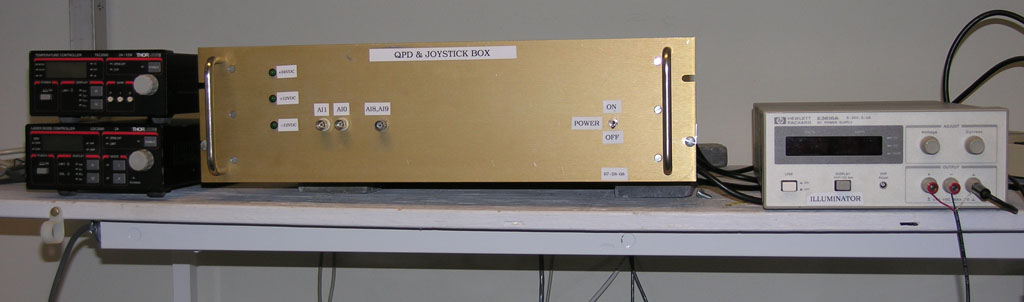
\includegraphics[width=\linewidth,keepaspectratio]{images/OTZ_Controls_0142B.jpg}}
    \caption{Electronic Controls. See larger image \href{http://experimentationlab.berkeley.edu/sites/default/files/images/OTZ_Controls_0142B.jpg}{\textbf{here}}}
\end{minipage}
\end{figure}

\begin{figure}[h]
\begin{minipage}{0.32\textwidth}
    \href{http://experimentationlab.berkeley.edu/sites/default/files/images/OTZ_0141B.jpg}{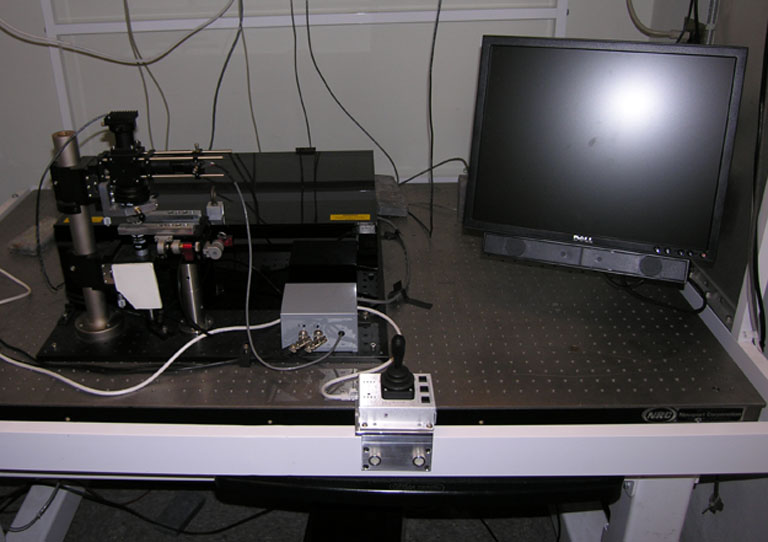
\includegraphics[width=\linewidth,keepaspectratio]{images/OTZ_0141B.jpg}}
    \caption{Optical Trap Setup. See larger image \href{http://experimentationlab.berkeley.edu/sites/default/files/images/OTZ_0141B.jpg}{\textbf{here}}}
\end{minipage}
\begin{minipage}{0.32\textwidth}
    \href{http://experimentationlab.berkeley.edu/sites/default/files/images/OTZ_3551_Crop.jpg}{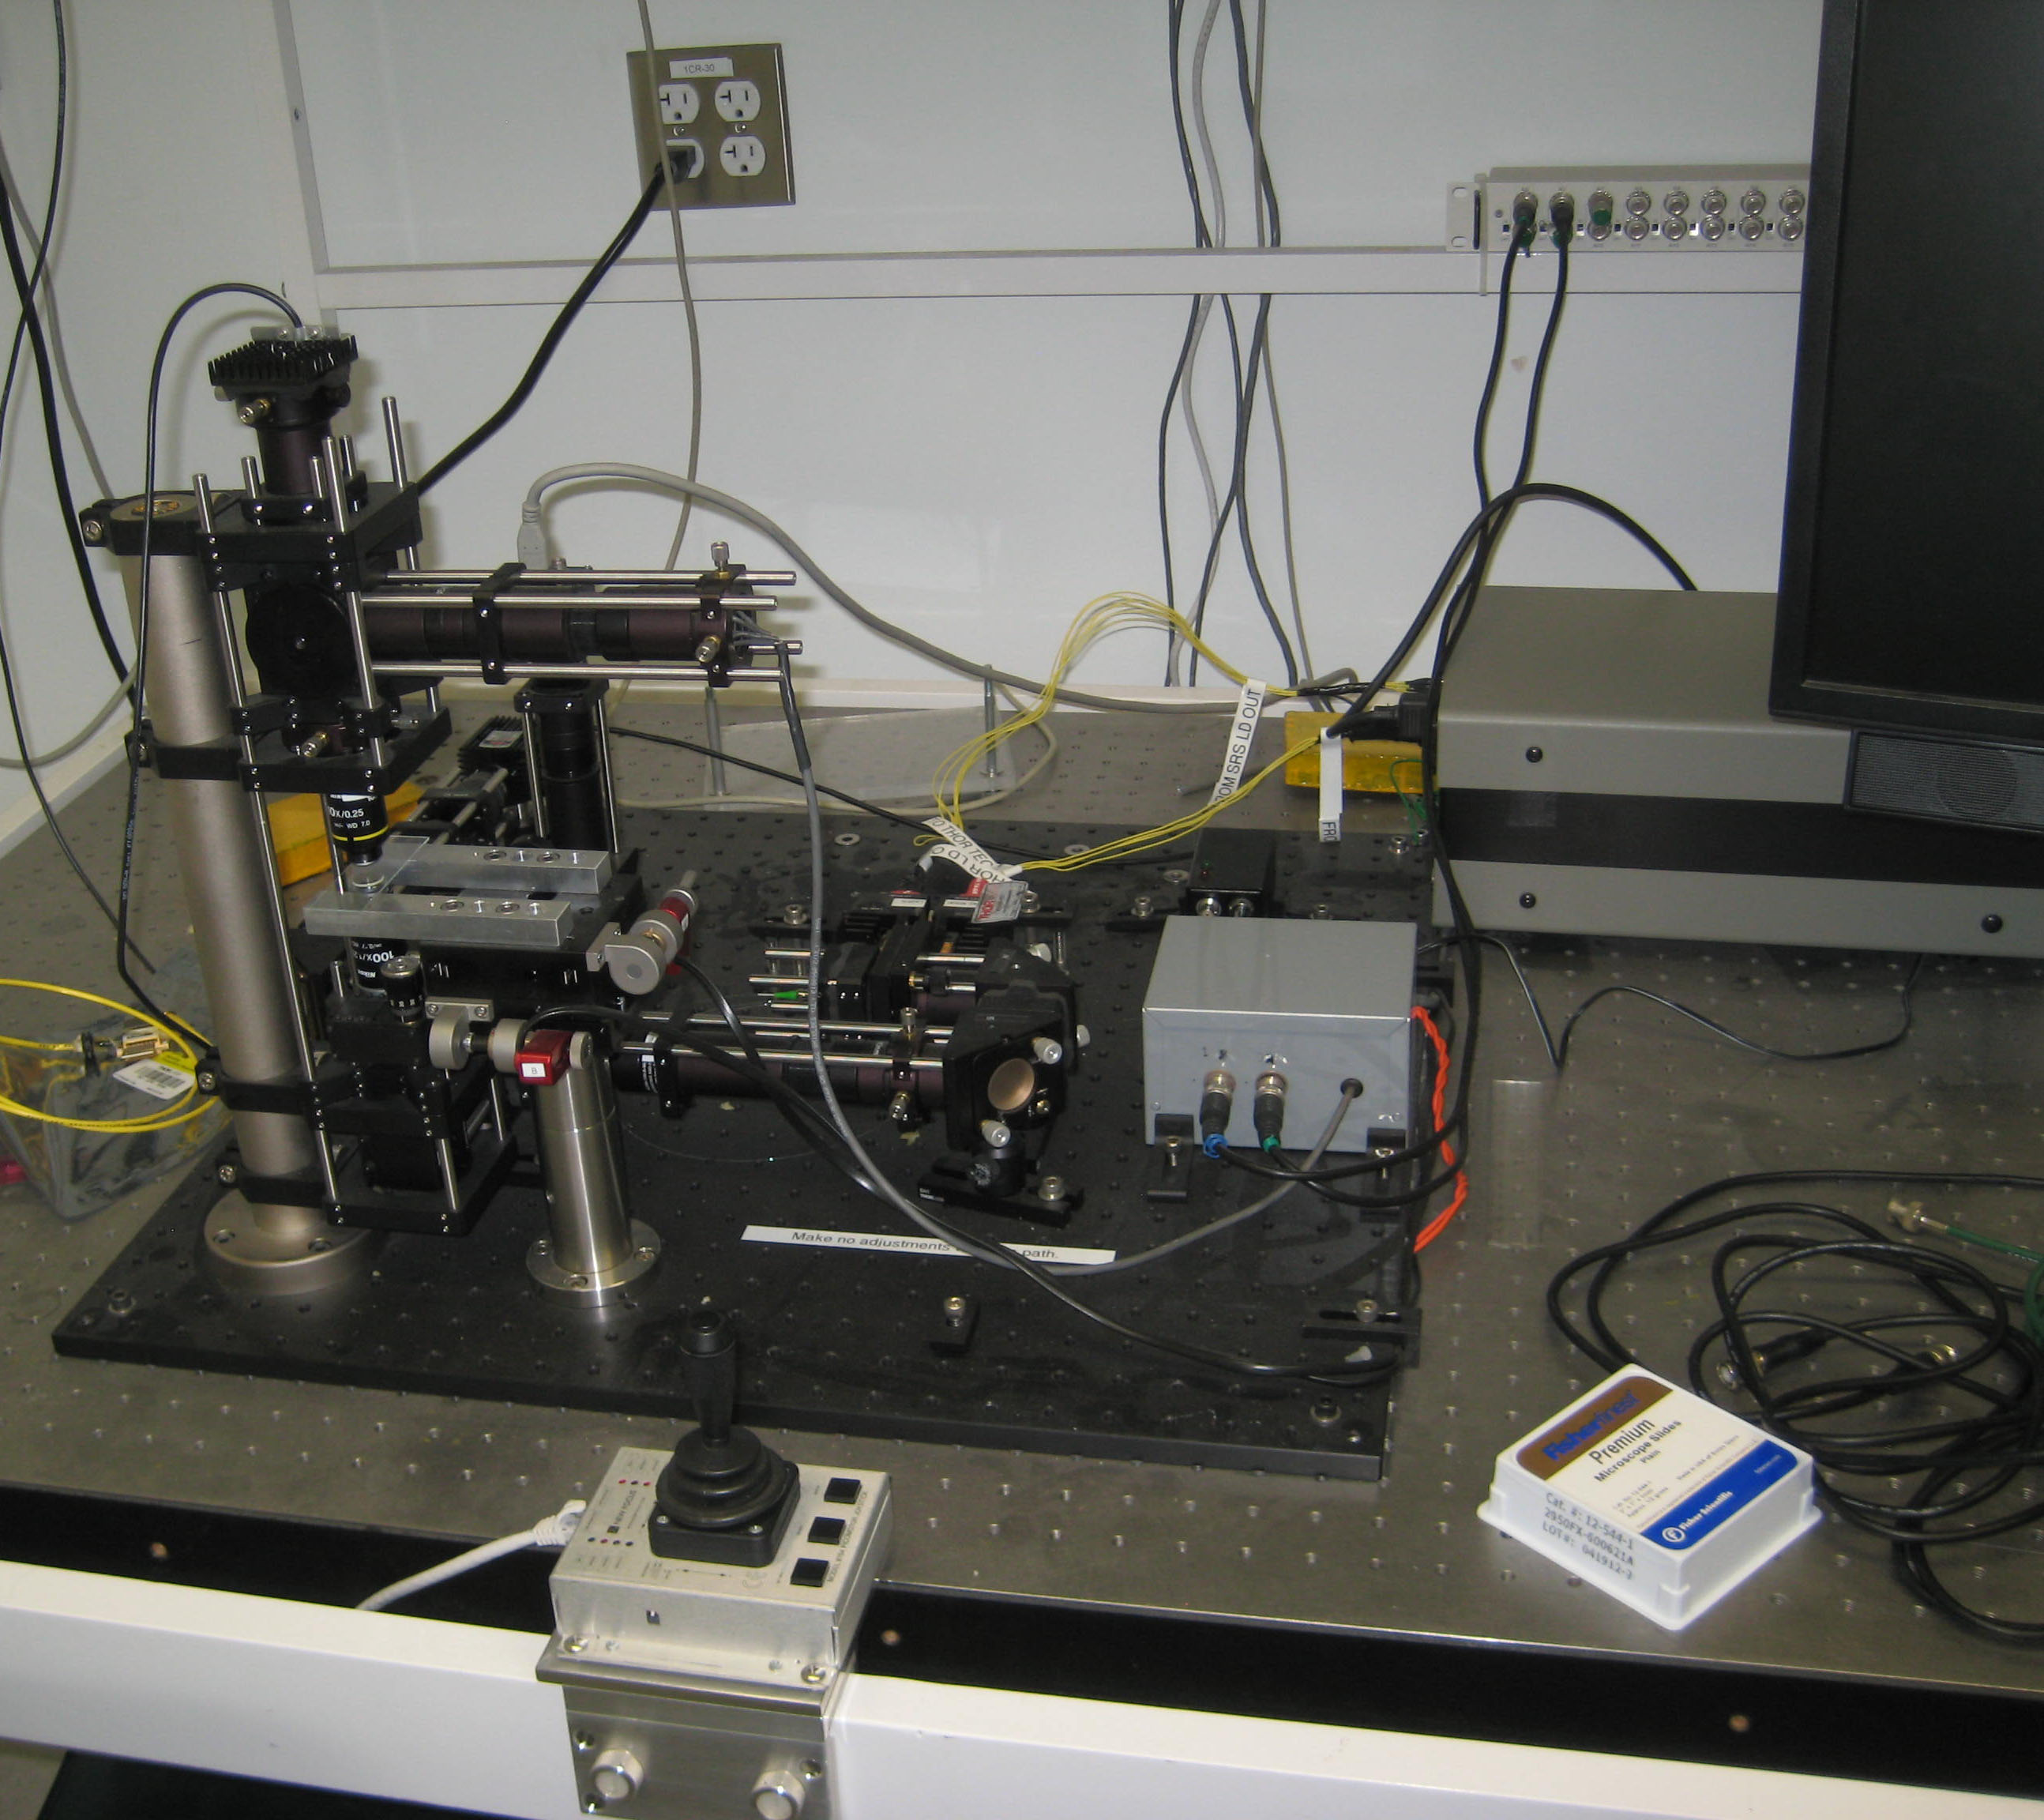
\includegraphics[width=\linewidth,keepaspectratio]{images/OTZ_3551_Crop.jpg}}
    \caption{OTZ Stage with Slide. See larger image \href{http://experimentationlab.berkeley.edu/sites/default/files/images/OTZ_3551_Crop.jpg}{\textbf{here}}}
\end{minipage}
\begin{minipage}{0.32\textwidth}
    \href{http://experimentationlab.berkeley.edu/sites/default/files/images/OTZ_DAQ_Interface_3554.jpg}{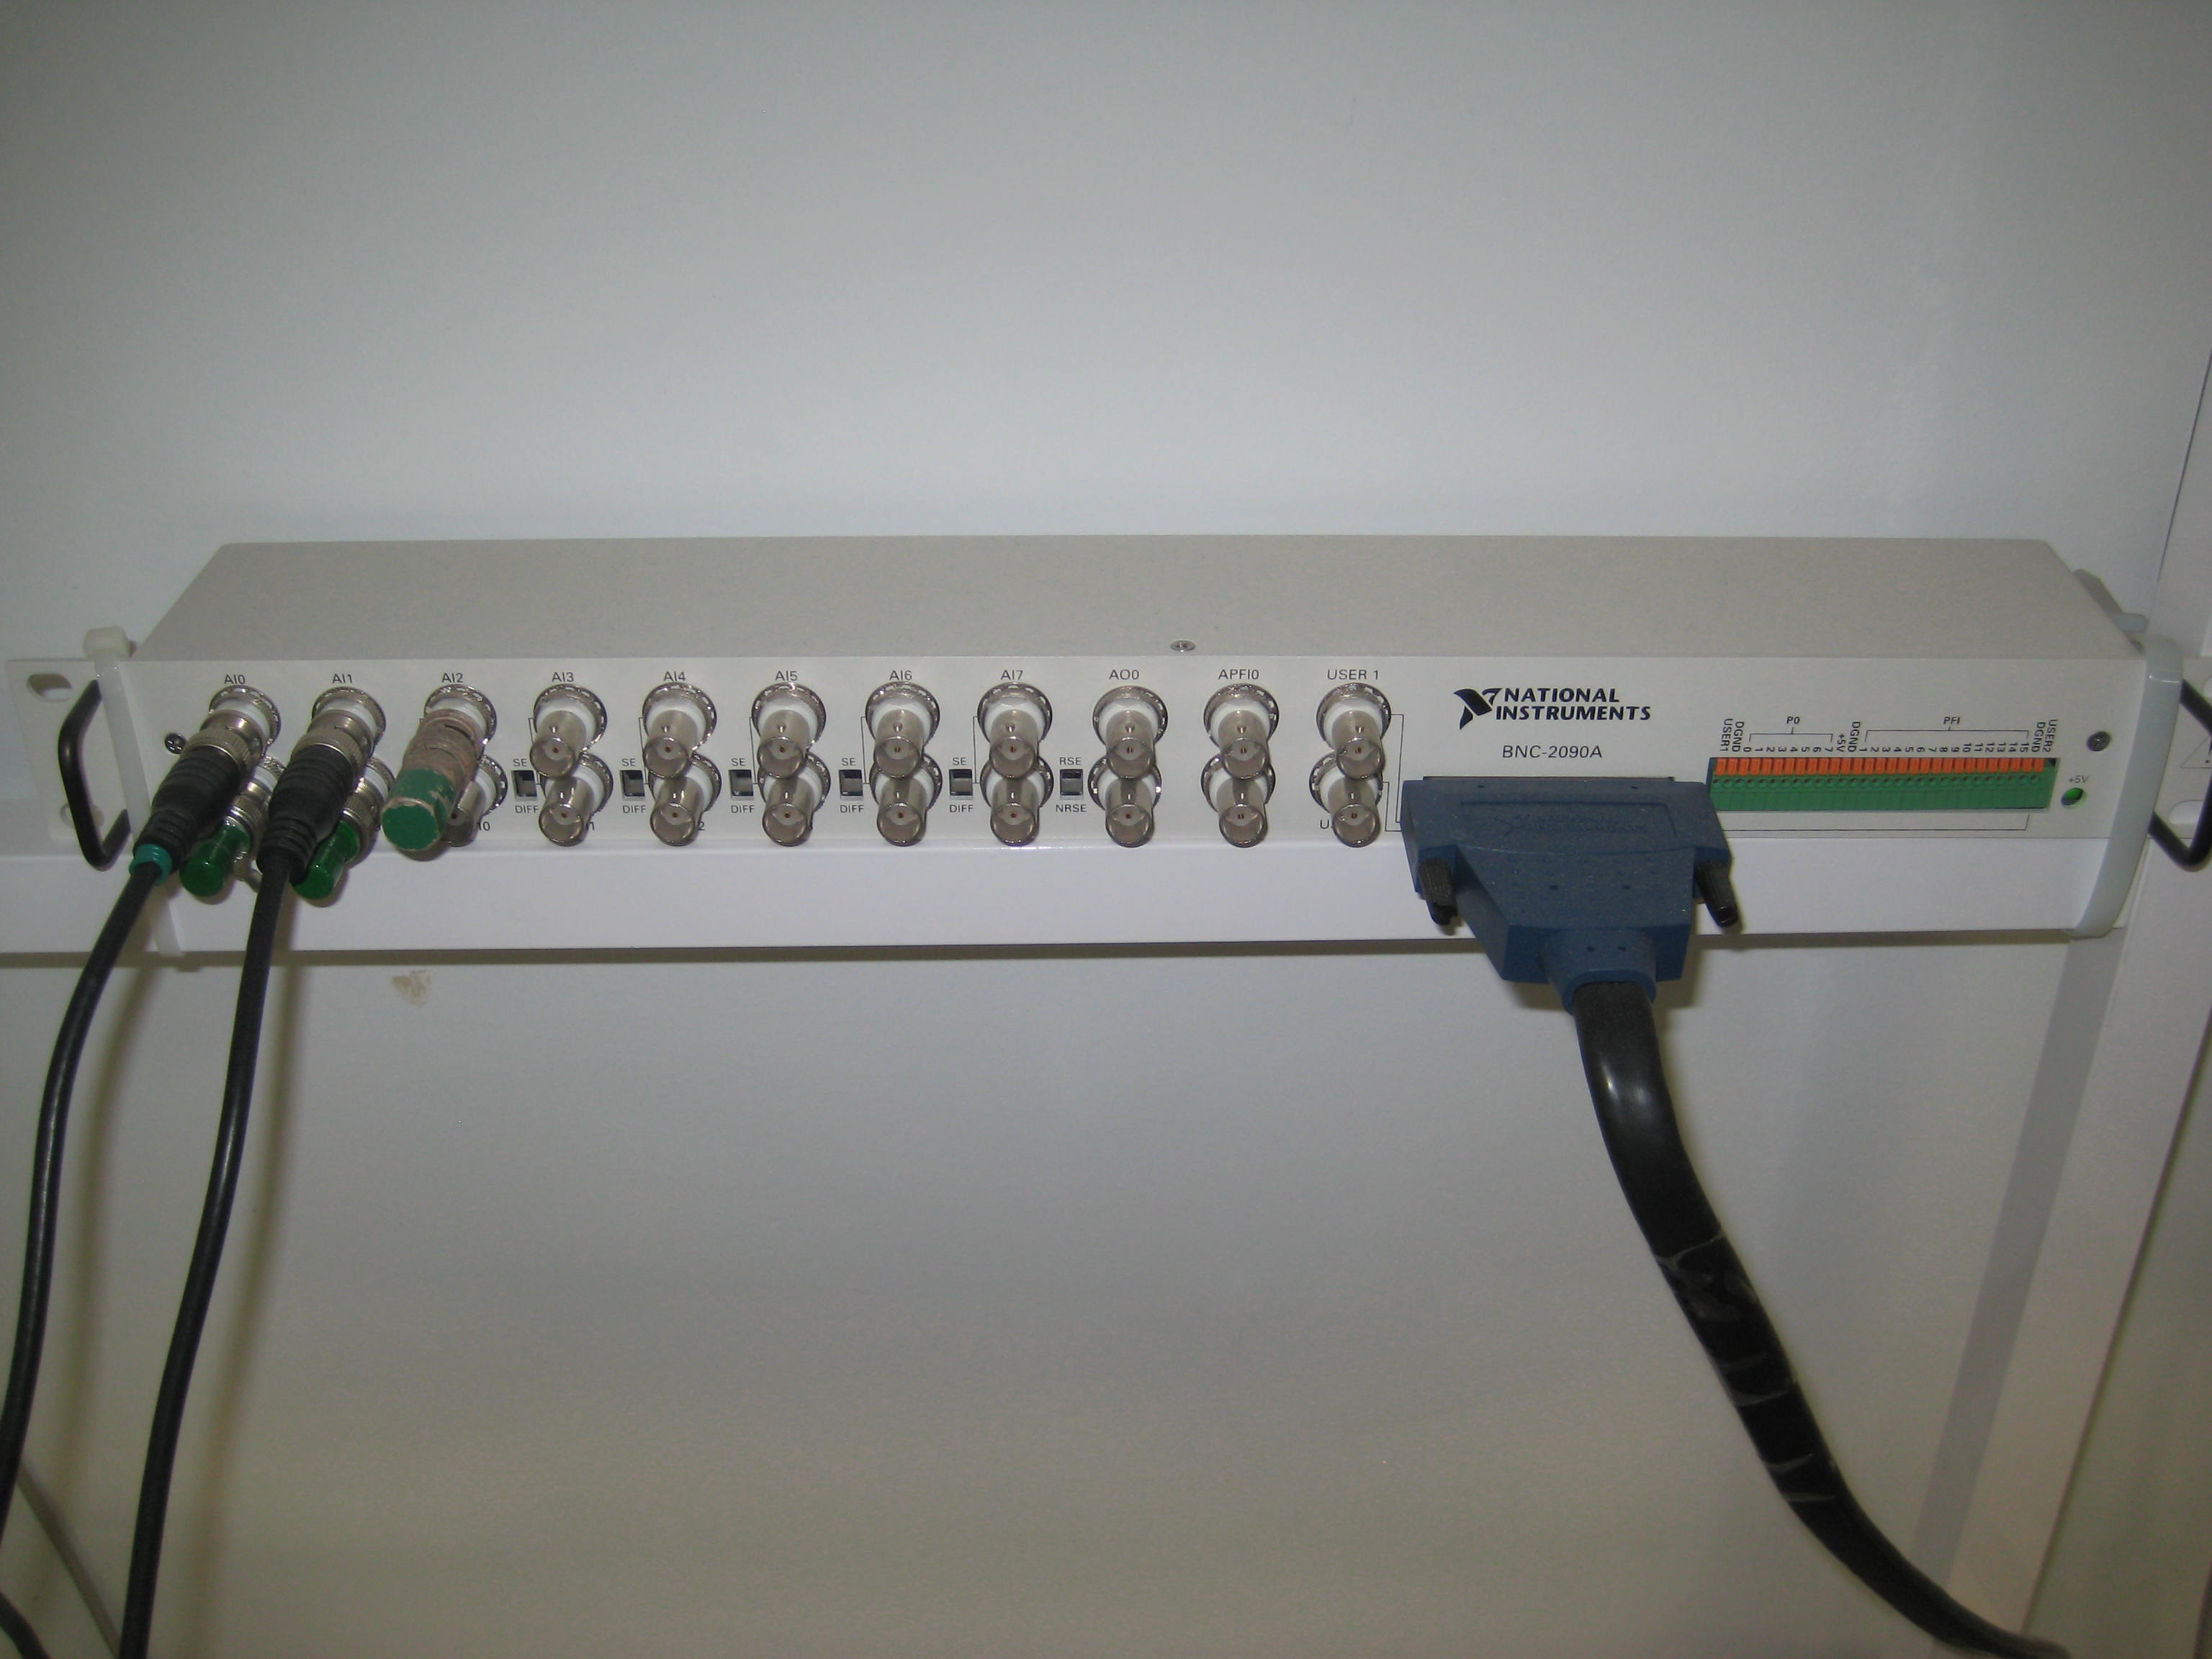
\includegraphics[width=\linewidth,keepaspectratio]{images/OTZ_DAQ_Interface_3554.jpg}}
    \caption{DAQ Interface Box. See larger image \href{http://experimentationlab.berkeley.edu/sites/default/files/images/OTZ_DAQ_Interface_3554.jpg}{\textbf{here}}}
\end{minipage}
\end{figure}

\begin{figure}[h]
\begin{minipage}{0.32\textwidth}
    \href{http://experimentationlab.berkeley.edu/sites/default/files/images/OTZ_Table_3555.jpg}{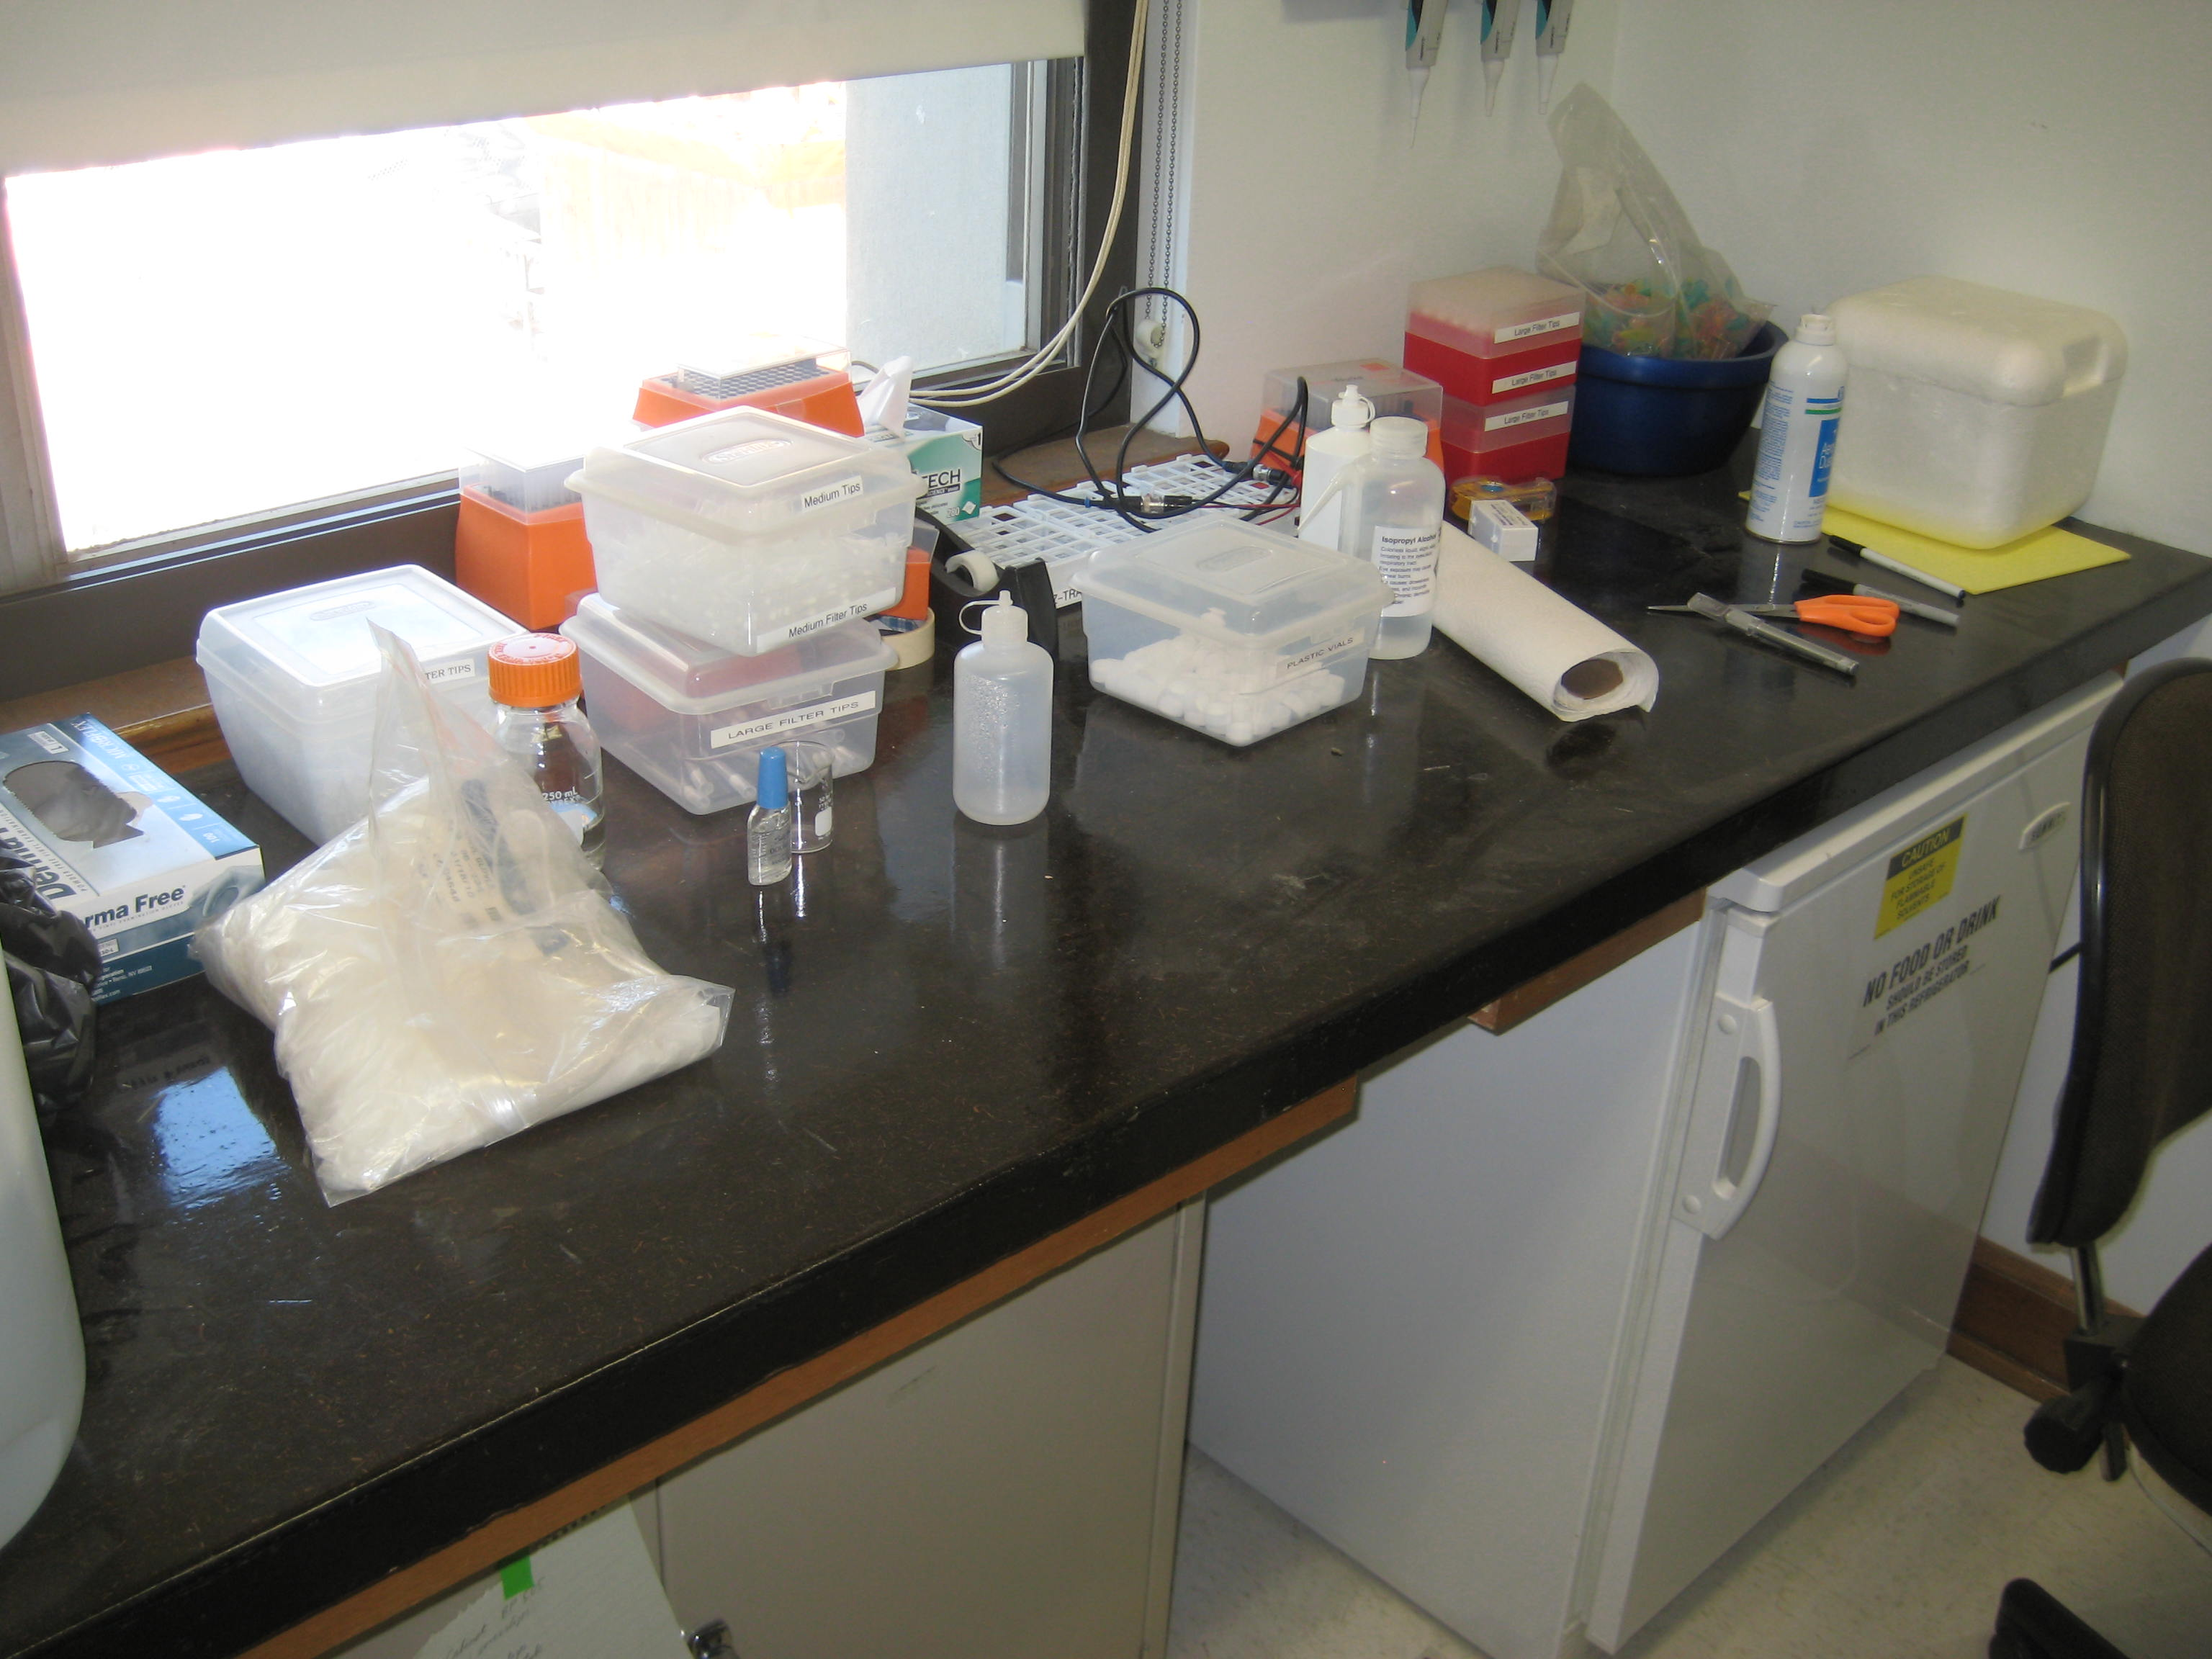
\includegraphics[width=\linewidth,keepaspectratio]{images/OTZ_Table_3555.jpg}}
    \caption{Sample Prep Table. See larger image \href{http://experimentationlab.berkeley.edu/sites/default/files/images/OTZ_Table_3555.jpg}{\textbf{here}}}
\end{minipage}
\begin{minipage}{0.32\textwidth}
    \href{http://experimentationlab.berkeley.edu/sites/default/files/images/OTZ_Laser_Controller_3553.jpg}{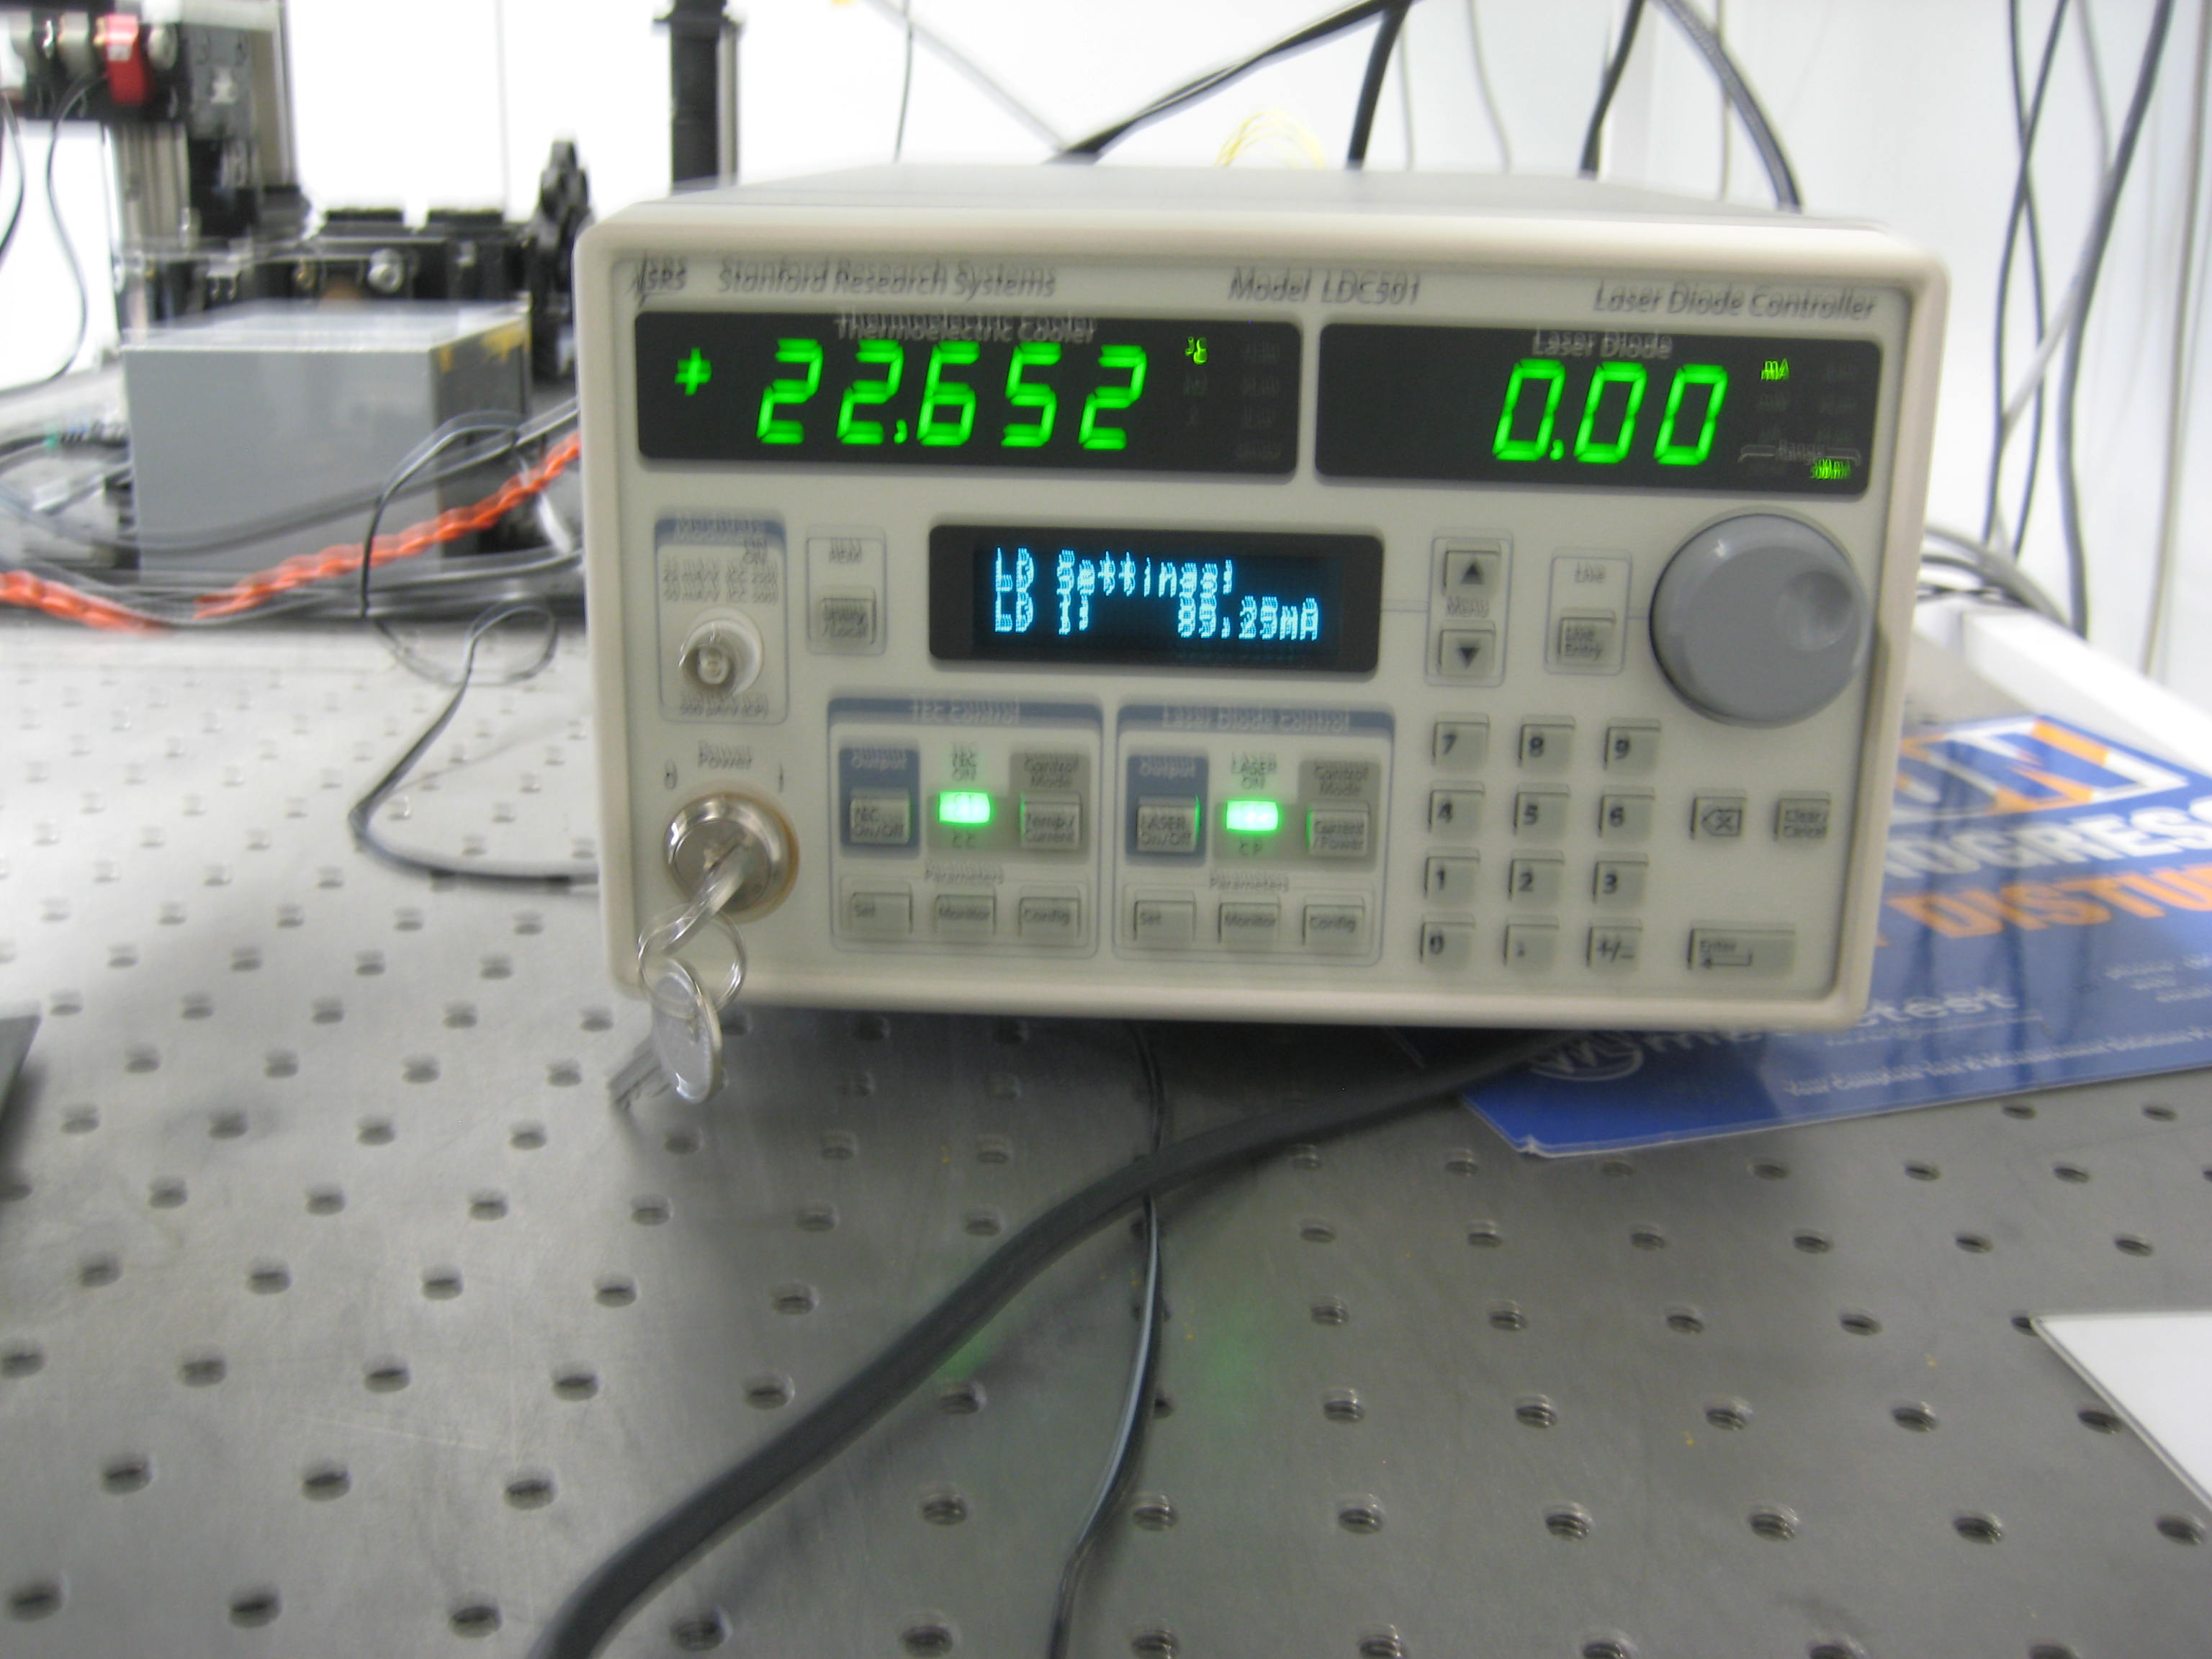
\includegraphics[width=\linewidth,keepaspectratio]{images/OTZ_Laser_Controller_3553.jpg}}
    \caption{Laser & TEC Controller. See larger image \href{http://experimentationlab.berkeley.edu/sites/default/files/images/OTZ_Laser_Controller_3553.jpg}{\textbf{here}}}
\end{minipage}
\begin{minipage}{0.32\textwidth}
    \href{http://experimentationlab.berkeley.edu/sites/default/files/images/OTZ_Laser_3550.jpg}{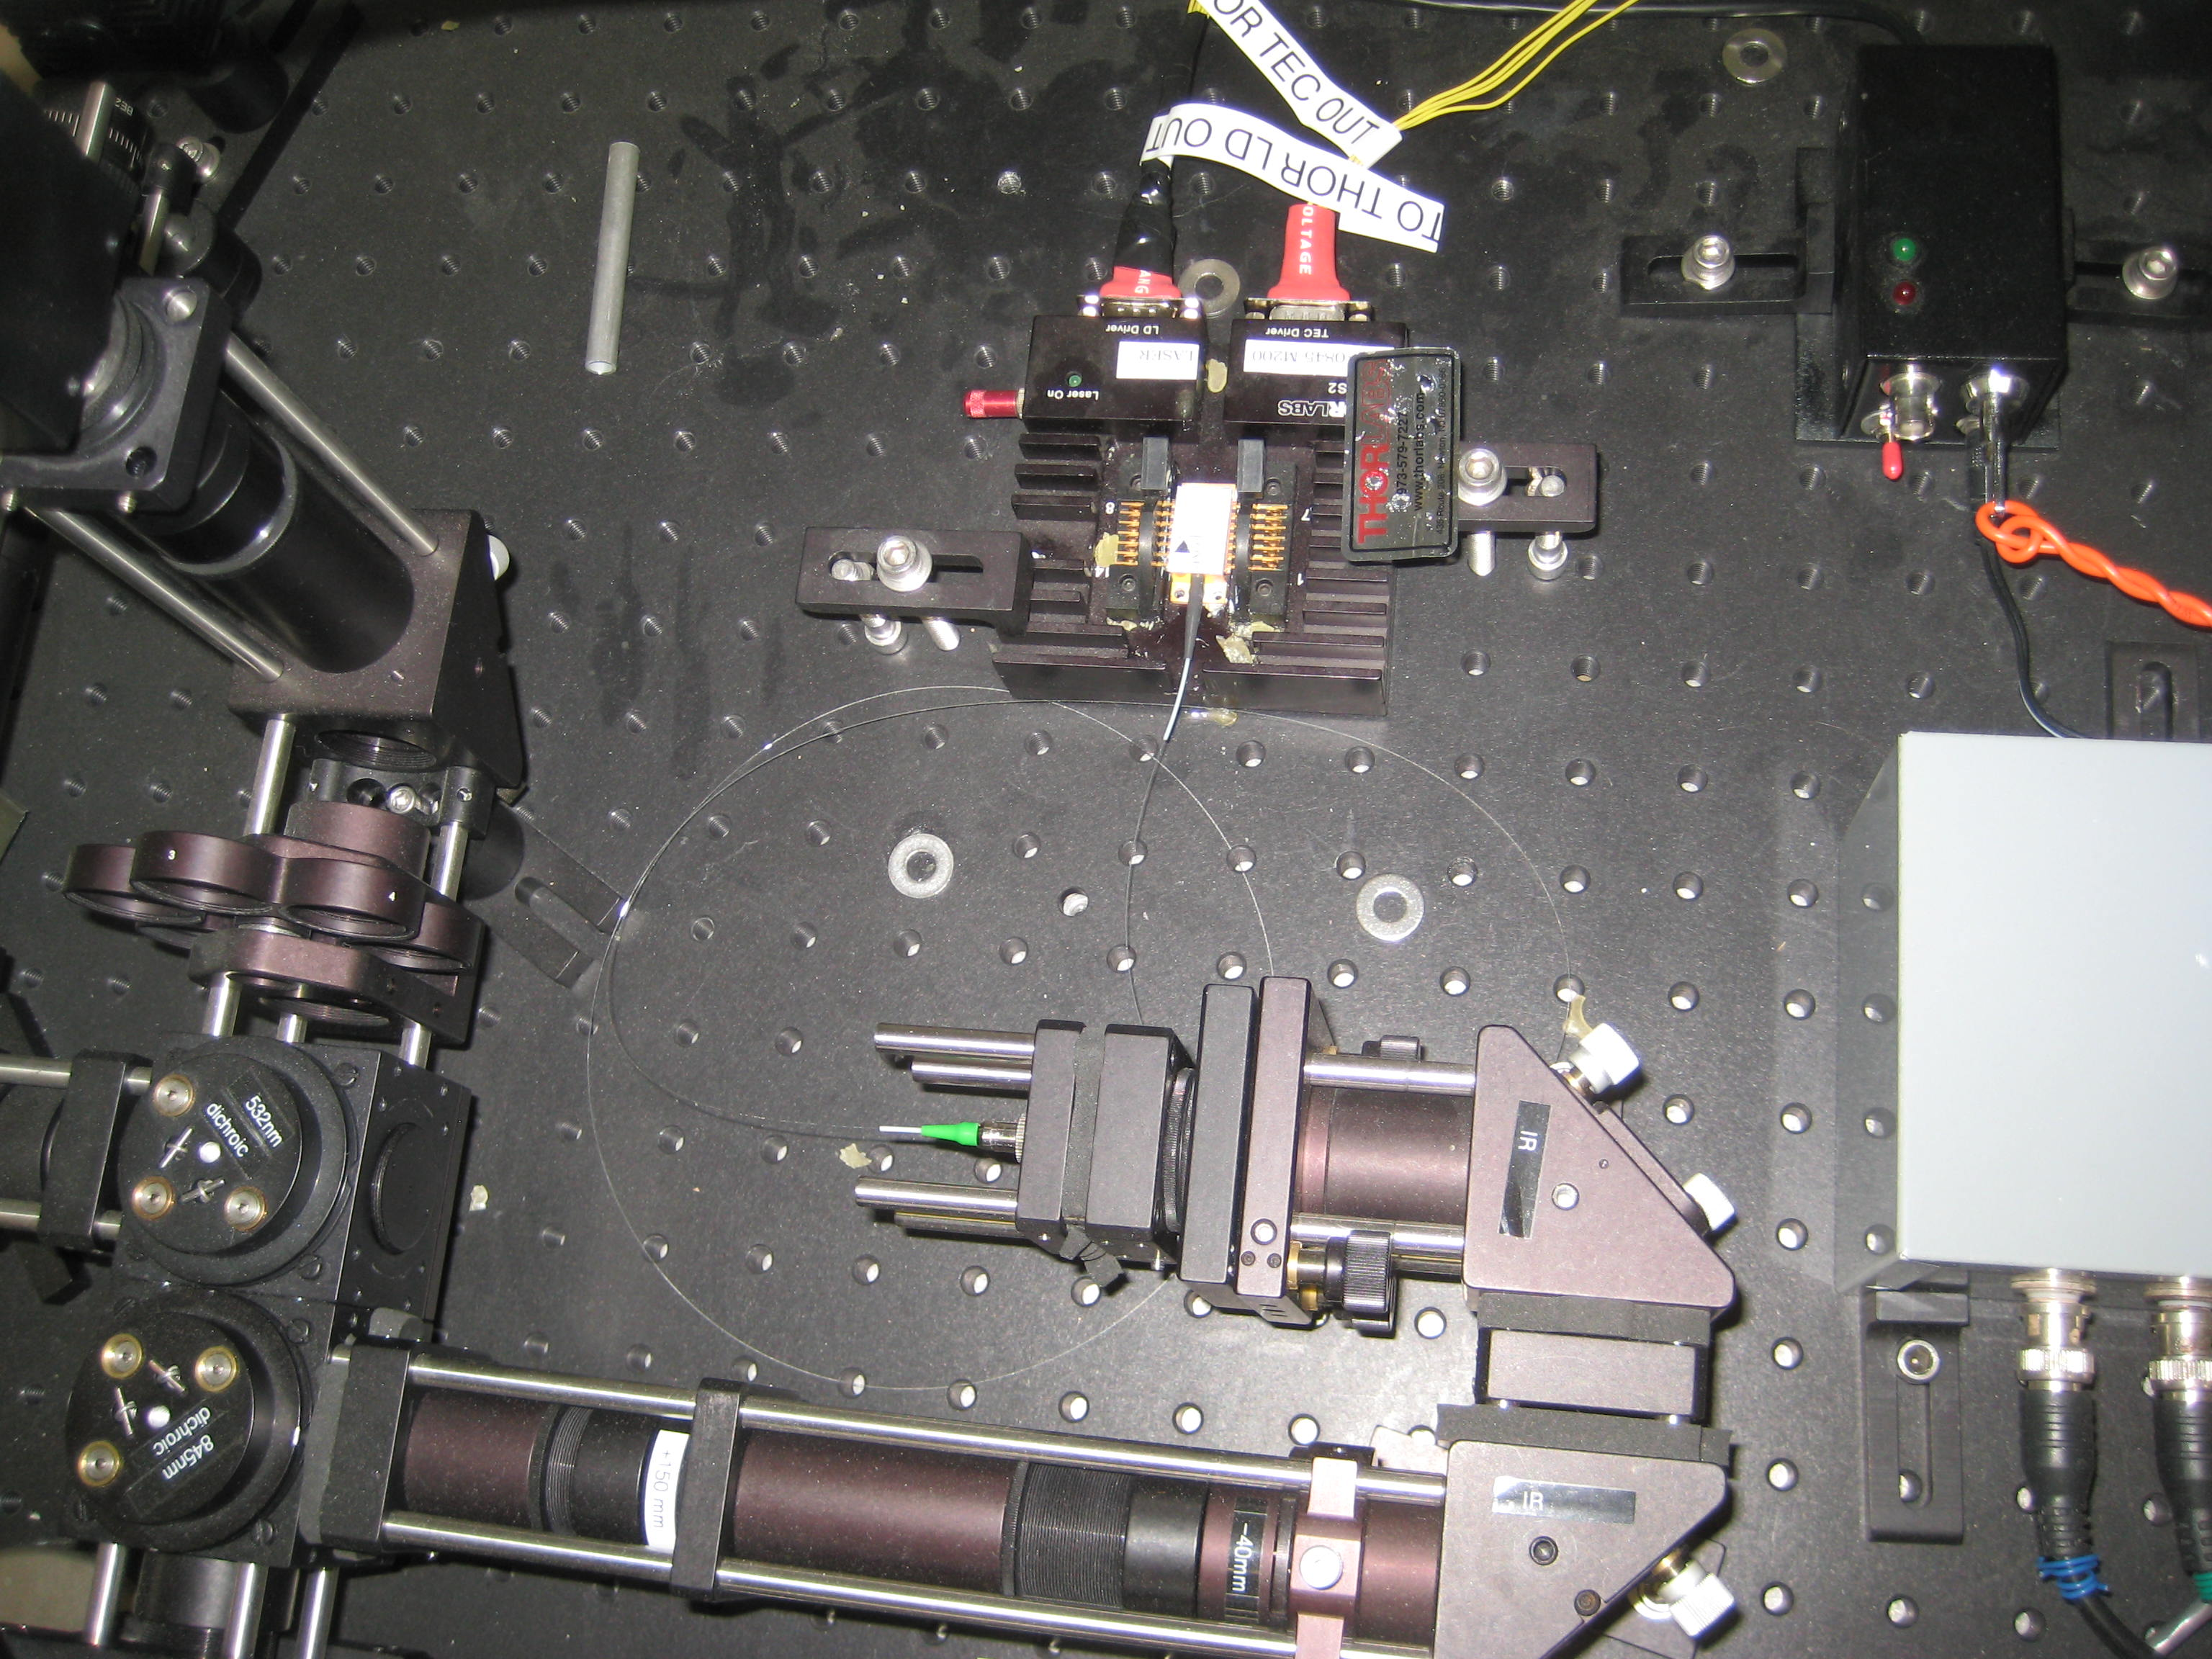
\includegraphics[width=\linewidth,keepaspectratio]{images/OTZ_Laser_3550.jpg}}
    \caption{945 nm Laser. See larger image \href{http://experimentationlab.berkeley.edu/sites/default/files/images/OTZ_Laser_3550.jpg}{\textbf{here}}}
\end{minipage}
\end{figure}

\section{Before The 1st Day of Lab}

\textbf{Complete the following before your experiment's scheduled start date:}

\begin{enumerate}
    \item Complete the training in the safe use of lasers detailed on the \href{http://experimentationlab.berkeley.edu/LaserSafety}{\textbf{Laser Safety Training}} page. This includes readings, watching a video, taking a quiz, and filling out a form.

    \item Watch the \href{http://youtu.be/bqIBcjcAhso}{\textbf{Optical Tweezer video}}.

    \item Check points are examination points that are placed in this lab where you must STOP and call a GSI or professor to make sure you understand what's expected. There could  be multiple check points throughout your lab so make sure you don't skip them since there is a \href{http://experimentationlab.berkeley.edu/otzcheckpoints}{\textbf{sign off sheet}} that must be turned in with your lab report. There are 6 Checkpoints in this lab.

    \item Complete the \href{http://experimentationlab.berkeley.edu/OTZprelab}{\textbf{OTZ Pre Lab and Evaluation}} sheets. Print, fill it out, then turn in with your answers. The Pre-Lab must be printed separately. Discuss the experiment and pre-lab questions with any faculty member or GSI and get it signed off by that faculty member or GSI. Turn in the signed pre-lab sheet with your lab report.

    \item Read this lab write-up through the end of \emph{Part I. Calibration of the Optical Trap}

    \item Last day of the experiment please fill out the \href{\ExperimentEvaluation}{\textbf{Experiment Evaluation}}

    \item \textbf{NOTE: LASER  SAFETY eyewear is required to be worn at ALL times during this experiment.}

\end{enumerate}

\textbf{Suggested Reading:}

\begin{enumerate}
    \item Read K. C. Neuman and S. M. Block, ``\href{http://physics111.lib.berkeley.edu/Physics111/Reprints/OTZ/Neuman-optical_Trapping.pdf}{\textbf{Optical Trapping}},'' Rev. Sci. Instrum. \textbf{75}, 2787 (2004). Pay particular attention to the overview and theory of of optical trapping and the sections on calibration techniques. You may also refer to the Wikipedia article \href{http://en.wikipedia.org/wiki/Optical\_tweezers}{\textbf{Optical Tweezers}}. Note: as a Wikipedia article the information is subject to change and may not be completely accurate, browse at your own risk. Use this \href{http://physics111.lib.berkeley.edu/Physics111/Reprints/OTZ/biowikipedia.pdf}{\textbf{definitions sheet}} instead.

    \item Go over \href{http://experimentationlab.berkeley.edu/sites/default/files/images/LDC501m.pdf}{\textbf{SRS-LDC501 Laser \& TEC Controller Manual}} to get familiar with the operation of this controller.

\end{enumerate}

You should keep a laboratory notebook. The notebook should contain a detailed record of everything that was done and how/why it was done, as well as all of the data and analysis, also with plenty of how/why entries. This will aid you when you write your report.

\section{Objectives}

\begin{itemize}
    \item Learn what real experimental physics is about

    \item Learn the synergy between experimental and theoretical work

    \item Learn to use pieces of equipment that are commonly used in research

    \item Learn how measurements are performed, analyzed, and interpreted.

    \item Learn how to present your work and results

    \item Learn problem solving strategies

    \item Learn how to manage and organize your time
\end{itemize}

\section{Introduction}

\subsection{What is an Optical Trap?}

An optical trap, or laser tweezers, is a device used to apply pico-newton sized forces and make precise measurements on a scale of roughly one micron. The trap is created by focusing a laser onto a dielectric material such as a silica bead or small living cell. The size and force scales make optical traps particularly useful in studying biological systems. Cells and organelles within cells can be manipulated and sorted. The forces and step-sizes of individual motor molecules such as kinesin and myosin can be measured by using beads as convenient handles to tug on and follow motors moving along cytoskeletal proteins. Optical traps are also used to study structural properties of cells, membranes, viruses, and DNA.

Arthur Ashkin discovered the method of optical trapping in 1970 \cite{Ashkin1970,Ashkin1997}. He calculated that the momentum from a high power laser, focused entirely onto a micron bead would propel the bead forward with 100,000 g's of acceleration. Taken by curiosity he performed this experiment and found that not only was the intended bead pushed downstream by the laser but also that other beads in his solution were highly attracted to the beam-path and flew in laterally from other parts of his slide. He then created the first working trap by using two opposing laser beams. At one point a bacterium that had contaminated a sample flew into the trap and was trapped, thus instigating the trap's revolutionary use in cell biology. Today optical traps are used extensively in both atom-trapping experiments and in biophysics labs worldwide. Faculty in Berkeley's Physics Department who use optical traps include Professors \href{http://physics.berkeley.edu/people/faculty/carlos-bustamante}{\textbf{Carlos Bustamente}}, and \href{http://physics.berkeley.edu/people/faculty/ahmet-yildiz}{\textbf{Ahmet Yildiz}}.

\subsection{The Physics Behind Trapping}

\begin{figure}[h]
    \centering
    \href{http://experimentationlab.berkeley.edu/sites/default/files/images/500px-Optical_Trap_Ray_Optics_Explanation.jpg}{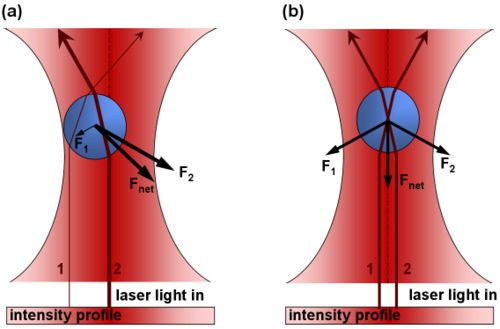
\includegraphics[width=0.5\linewidth]{images/500px-Optical_Trap_Ray_Optics_Explanation.jpg}}
    \caption{A ray diagram showing how the gradient force stabilizes the trap laterally}
    \label{fig:500px-Optical_Trap_Ray_Optics_Explanation}
\end{figure}

The most straightforward mechanism to understand the physics of trapping is to consider the change in momentum of light that is scattered by and refracted by a dialectic material, in our case a silica glass bead. Any change in the direction of light imparts momentum to the bead. This mechanism holds for objects much larger in diameter than the wavelength of the laser. A ray-tracing argument holds that the scattered light creates a \emph{scattering force} in the direction of light propagation, while the refracted light creates an opposing \emph{gradient force}. When the bead is in the center of the trap, these forces cancel. When a bead moves slightly away from the center, a net force is applied towards the center, making this a stable equilibrium.

\newpage

In order to understand how the equilibrium is stable, it will help to consider how the gradient force responds to displacement of a bead from the center. In the figure to the right, the red region represents the ``waist'' of the laser at its focus point, with the laser passing upward through the sample chamber. The blue ball is the bead, and the black arrows (1) and (2) represent light rays whose thicknesses correspond to their intensities (note that the beam is brightest at its center). In case (a), with the particle slightly to the left of center, the two rays refract through the particle and bend inwards. The reactionary force vectors, F1 and F2, of each ray on the bead are shown. Because ray (2) is more intense (and thus carries more momentum) than ray 1, the net force on the bead is to the right. Thus, a perturbation to the left causes a rightward-directed force back towards the trap's center.

In case (b) the particle is centered laterally in the beam and will not be pushed left or right. The net gradient force is downward, which is balanced by an upward scattering force (not shown) due to reflection of some of the light.

To better understand how the scattering and gradient forces and the trap's stability vary with bead displacement both vertically and horizontally, try this \href{http://glass.phys.uniroma1.it/dileonardo/content/apps/trapforces.php}{\textbf{Java applet}} from the Di Leonardo lab \cite{Leonardo} in Italy. The model used for this applet shows the importance of a high numerical aperture lens, as the extremal rays illustrated contribute disproportionately to the change in gradient force vertically. (Note that you must adjust the numerical aperture at the bottom of the applet in order to obtain a stable trap.) By moving the bead around and looking at the net force vector, you can get a pretty good feel for how the restoring force varies as a bead is displaced horizontally or vertically from the trap's center. Note particularly how the trap is less stiff as the bead is displaced above the trap's center. Remember this when you trap your first bead and try moving the bead with the stage and focus controls.

The ray optics approach described above holds for trapped objects whose diameter is much larger than the wavelength of the laser. For objects much smaller than this wavelength, ray optics are not valid. In this case, conditions for Raleigh scattering are satisfied and the object can be treated as a point dipole. The scattering force then is due to absorption and reradiation of light by the dipole, and the gradient force arises from the interaction of the induced dipole with an inhomogeneous electromagnetic field. This mechanism is detailed in the Neuman and Block review \cite{Neuman}. Use this \href{http://physics111.lib.berkeley.edu/Physics111/Reprints/OTZ/biowikipedia.pdf}{\textbf{definitions sheet}} as needed. More complicated electromagnetic theories have been invoked to account for the observed forces \cite{Neuman,Bechhoefer,Shaevitz}. However, these theories are not particularly useful in calculating forces from first principles; the ray optics approach is useful for guiding trap design and beam alignment, while calibration is based on direct measurements of bead motion.

\subsection{Experiment Timeline}

\textbf{NOTE: LASER  SAFETY eyewear is required to be worn during this experiment.}

\textbf{Days 1 and 2}

\begin{itemize}
    \item Learn to trap beads and collect data for calibrations

    \item Tell Don Orlando or Amin Jazaeri what day (if any) you want to start working with \emph{E. coli} so that cultures can be started three days before (so not available on Mondays). You should be requesting the cultures roughly on your second day.
\end{itemize}

\textbf{Day 3}

\begin{itemize}
    \item Analyze calibration data enough to show that you have good data and understand how to analyze.

    \item Read the \emph{E. coli}  references and consider what how to investigation what you want to do. You will complete two experiments (Internal Transport in Onions (you supply it), or \emph{E. coli} Locomotion ( must give three-day notice)
\end{itemize}

\textbf{Days 4-5}

\begin{itemize}
    \item Complete the first experiment.
\end{itemize}

\textbf{Days 6-7}

\begin{itemize}
    \item Complete second experiment. Consider leaving more time for analysis.
\end{itemize}

\section{Apparatus}

The key to a successful optical trap is to create a well-collimated beam that slightly overfills the aperture of the microscope's objective lens and is aligned perfectly with the optical axis of the objective lens.

\begin{figure}[h]
    \centering
    \href{http://experimentationlab.berkeley.edu/sites/default/files/images/450px-OTZ_From_Above.gif}{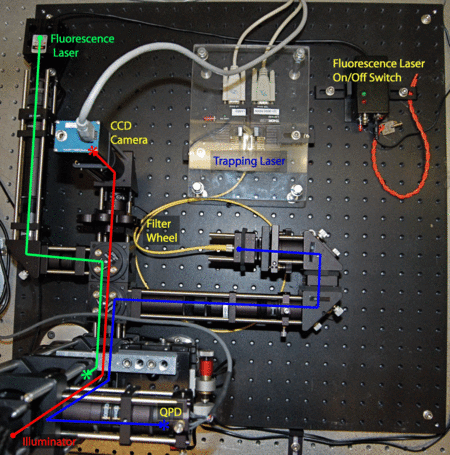
\includegraphics[width=0.5\linewidth]{images/450px-OTZ_From_Above.png}}
    \caption{Optical trap seen from above.}
    \label{fig:450px-OTZ_From_Above}
\end{figure}

The numerous mirrors and lenses that steer and shape the beam to this end require delicate alignment by a trained staff member with safety goggles, an IR viewer, and special tools. \textbf{Do not tamper with anything in the laser beam path unless specifically instructed!} Even a slight nudge of a mirror or lens can result in an asymmetric or off-center beam that will ruin the function of the trap and require hours of realignment. (If you're curious about the process, see the \href{http://experimentationlab.berkeley.edu/DesignandDocumentationOTZ#Laser\_Alignment\_and\_Collimation}{\textbf{laser alignment and collimation procedure}}, but don't do any of this yourself!) If there is any problem with the function of the trap itself, notify the staff and do NOT try to fix it.

\textbf{Beam Path}

From the 975 nm laser it goes through two steering mirrors, then 1/2 waveplate at 980nm bandpass, (DO NOT ADJUST or TURN IT) then goes through lens, then to the 950nm Shortpass Dichoric mirror. With the addition of the point Grey camera, we needed to remove the Shott filter KG-5, but the FG900 filter is still installed.

\subsection{Lasers}

\subsubsection{Trapping Laser}

\newpage

The Axcel from Thorlabs BF-979-0300 300mW Max diode laser \href{http://experimentationlab.berkeley.edu/sites/default/files/images/975nm-Laser-Specs.pdf}{\textbf{975nm Laser Specs}} This has a maximum power output of 300 mW, though a fraction is lost traveling through all the optics. The 975nm wavelength is far enough from the resonant frequency of water to prevent much heating of live cells and is less likely to affect the behavior of cells than visible wavelengths. The diode laser is coupled to a very very delicate optical fiber. DO NOT TOUCH IT!!! If this fiber is broken or kinked it could cause backwards reflections of the beam, destroying the laser. The laser diode is mounted in a standard butterfly mount that acts as a heat sink and cooling device. Two cables connect it to a laser diode controller \href{http://experimentationlab.berkeley.edu/sites/default/files/images/LDC501m.pdf}{\textbf{LDC 501 Laser Controller full Manual}} and thermoelectric temperature controller (TEC) located on a shelf above the optical table. Avoid touching the laser or its butterfly mount because static discharge can destroy the laser and the fibre is very very small. \href{http://experimentationlab.berkeley.edu/sites/default/files/images/SOP\_Laser\_Diode\_Driver.pdf}{\textbf{The getting started SOP for this Laser controller}} See References below for SRS controller cable wiring diagram.

\subsubsection{Fluorescence Laser}

The smaller laser is an over-the-counter, $<$5mW, 532nm diode laser. It is just as dangerous as the average green laser pointer, so as long as you don't look into the beam you will remain sighted.

\subsection{Safety Measures}

The trapping laser has a power output of up to 300 mW and a wavelength of 975nm, which is in the near infrared. Even a brief exposure to the focused beam at this power can cause permanent damage to the retina of your eye. Because the beam is invisible, you could be exposed without even realizing it. For this reason, the beam path is shielded. Still, the laser safety training and measures below are essential for your protection.

\textbf{NOTE: LASER  SAFETY eyewear is required to be worn at ALL times during this experiment.}

\begin{enumerate}
    \item Do not operate the laser unless you have completed the laser safety training and submitted the signed laser safety form and quiz to the course staff.

    \item Never bypass any safety devices, e.g. NEVER REMOVE A LENS TUBE.

    \item \textbf{Turn off} the trapping laser before putting oil on the objective lens or placing/removing a slide on the stage. The beam path can be deflected and focused through the oil, resulting in a safety hazard.

    \item Check for stray beams: Every day, the first time you turn on the trapping laser you should perform a survey of the beam around the objective to check if there are any stray beams (diffuse or specular) coming from any part of the laser or optics, and then document this in the Laser Log Book in wall pocket.

    \item The survey is done by using the IR Viewer, if it is not in the room find a staff member to locate it. The IR viewer is blue and you use it with your goggles on. The laser beam is invisible and very powerful; the IR viewer allows you to see it, but even if you can't see it you can still be blinded.

    \item When the laser is at its maximum power, with LD I set to 490.00 mA, the power output about an inch from the stage is .4 mW and drops off with distance $r$ away from the stage like $1/r^2$. This is not powerful enough to cause damage to your eyes, especially if you are seated in your chair and not leaning in toward the equipment. However, within the optical path the laser emits about 238 to 300 mW of power, so make sure that you do not touch/adjust/insert any elements in the optical path which could diffract the beam. After you have checked for stray beams and when you are not adding oil or moving the slide, you do not need to wear the laser safety glasses.

\end{enumerate}

\subsection{Optical Paths}

\newpage

The microscope has a dual function. One is to allow us to see our specimen at high magnification by sending visible light through the specimen to a video camera. The other function is to focus the laser beam to create the optical trap and collect the laser light to focus it on a quadrant photodiode (QPD) that tells us how close the trapped object is to the trap's center. Keep in mind that there are three light sources, and though their paths coincide through much of the microscope they are still distinct, with distinct focal and afocal points. A useful concept for understanding microscopy optics is that of \href{http://www.microscopyu.com/articles/formulas/formulasconjugate.html}{\textbf{conjugate planes}}, which groups all the optics into two complementary sets: imaging and illumination.

\textbf{Trapping Laser}

The trapping beam exits the diode and travels through a fiber optic cable to a cable termination fitting, then through a collimating lens. It then passes through two steering mirrors and a beam expander that expands the diameter 2.5x to match the 6 mm aperture of the microscope objective. It joins the microscope at a dichroic mirror, which reflects IR light but allows visible wavelengths to pass through. A mirror at the bottom front of the microscope reflects the beam up through the objective lens, which focuses the beam down to a tiny waist just above the lens, creating the trap. Above this waist, the beam diverges and is recollimated by a condenser lens. Above the condenser the beam is reflected off another dichroic mirror and focused by a lens onto the quadrant photodiode (QPD) for position detection.

\textbf{Illumination}

The trap has two illumination systems: the green laser and the red LED. The green laser is only used in the Dynein experiment, but regardless it is to your advantage to understand all parts of the apparatus, as it will only deepen your understanding.

\emph{LED Illuminator}

This is an inverted compound microscope, so it may be backwards from what you have used before. At the top is the illuminator, a red LED.

\begin{figure}[h]
    \centering
    \href{http://experimentationlab.berkeley.edu/sites/default/files/images/400px-Graphic1.jpg}{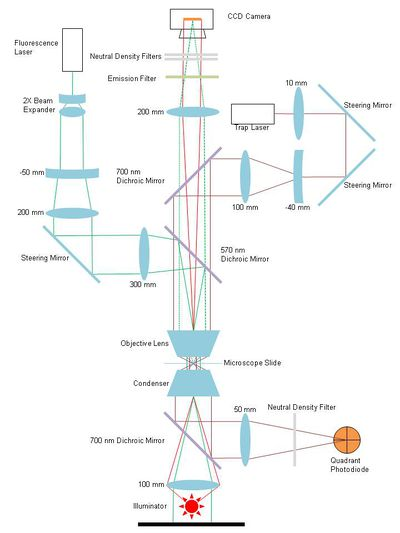
\includegraphics[width=0.5\linewidth]{images/400px-Graphic1.jpg}}
    \caption{The optical path. Illustrated with the emission filter in. Dotted green line represents emitted fluorescence.}
    \label{fig:400px-Graphic1}
\end{figure}

\begin{figure}[h]
    \centering
    \href{http://experimentationlab.berkeley.edu/sites/default/files/images/OTZ_From_Front.gif}{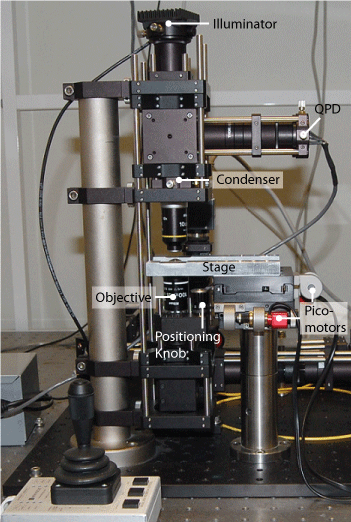
\includegraphics[width=0.5\linewidth]{images/OTZ_From_Front.png}}
    \caption{Inverted compound microscope, front view.}
    \label{fig:OTZ_From_Front}
\end{figure}

The light passes straight through a dichroic mirror and is focused on the condenser, which collimates it, giving even illumination of the sample. As it then passes through the objective lens the image is magnified by 100x. The mirror below the objective reflects the light to the dichroic mirrors (and emission filter if it's in), which allow red light through. The light is focused by a 200mm lens (the ``eyepiece'' of the microscope), and bounced off a mirror onto the CCD camera.

\emph{Fluorescence Laser}

The fluorescence laser's alignment is less critical than the trapping laser's, since at the sample it provides broad illumination rather than a tight focus. This is why we can get away with mounting it on a post rather than the cage system. The beam exits the laser unit collimated and goes through 8x expansion (a 2x unit and a 4x pair of lenses). It bounces off one steering mirror and through a lens, which (after it reflects off a dichroic mirror) focuses it on the back focal plane of the objective, which collimates it to provide the nice, even illumination we want. The condenser refocuses it, and then it passes through the QPD's dichroic mirror. The illuminator acts as a beam stop.

\emph{Fluorescent dye emission}

The dye fluoresces in every direction, but the part we are interested in goes through the objective (where it is magnified), off a mirror and through both dichroics and a lens for focusing. It then passes through the emission filter, which is a very tight bandpass to block everything except the dye's emission (which peaks at 570 nm) and the LED. Finally its journey is over when it reaches the CCD focused.

\newpage

\subsection{Stage}

\emph{\textbf{Make sure you do NOT turn or run the pico-motors to the ends of their rotation, they will jam up.}}

The microscope stage holds the specimen slide and allows fine control over horizontal positioning. It is useful for finding beads or cells to trap and moving them once trapped. Two piezo electric picomotors drive the stage in the X and Y directions. The knurled knob on each pico-motor allows for manual positioning. The motors can be controlled by a joystick or by software. The joystick is best for hunting for specimens to trap and moving the trapped specimens around. The software control is useful for calibration procedures when you want to move the slide at a constant speed. The specimen is held on the stage between a microscope slide and a thin glass coverslip suspended beneath.

Vertical positioning (Z axis) is accomplished by moving the objective lens with the positioning knob; 1$\mu$m/gradation. This has the effect of moving both the plane of focus of the microscope and the center of the optical trap. So, for instance, if you focus on a bead resting on the coverslip, turn on the laser to trap it; you can then move the objective lens up to raise the bead off the coverslip. This can be difficult in practice. When you turn the positioning knob take special care to not bump the microscope in any other way. This can bump the trapped bead out of the trap. Use two fingers only and do not rest your hand in anyway on the microscope.

The gap between the coverslip and objective lens is filled with immersion oil which, by virtue of its high(er than air's) refractive index, improves both the resolution and the numerical aperture of the lens.

\subsection{Quadrant Photo-Diode (QPD)}

\begin{figure}[h]
    \centering
    \href{http://experimentationlab.berkeley.edu/sites/default/files/images/350px-QPD2.jpg}{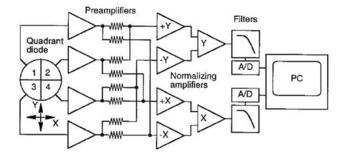
\includegraphics[width=0.5\linewidth]{images/350px-QPD2.jpg}}
    \caption{Schematic of the Quadrant Photo Diode position detection system. The signal from the diodes are amplified by low-noise preamplifiers and then networked to calculate the X and Y position of the incident light beam. The figure above, depicting the block diagram, is taken from  Allersma et al.}
    \label{fig:350px-QPD2}
\end{figure}

The quadrant photodiode (QPD) is our principal way of collecting data on the position of the trapped particle relative to the center of the trap. This distance also tells us the force the trap exerts on the particle since force increases linearly with distance from the trap's center. Some simpler optical traps use the video camera image to provide position information, but a photodiode allows finer spatial resolution and much higher frequencies (we'll be collecting data at 12 kHz for power spectrum analysis -- compared with 30-500 Hz for video cameras).

The QPD consists of 4 photodiodes in a quadrant formation to allow X and Y position calculation. Within a certain range of light intensities, the output voltage of a photodiode scales linearly with the intensity of light incident upon the diode. The light incident upon each quadrant in the QPD generates a voltage. The analog circuitry then outputs a voltage $V_x$ and $V_y$ which are proportional to the actual X and Y position of the incident beam. As the light scatters in a predictable way off of the spherical beads, this information can be used to recover actual bead position within a narrow range around the center of the trap. Further information can be found in reference: Gittes and Schmidt.

With nothing in the trap (or a trapped bead exactly centered in the trap), the laser beam is tightly focused on the center of the QPD, giving $V_x$ and $V_y$ signals of zero. When a trapped bead moves slightly away from the center of the trap, the laser spot moves on the QPD, causing $V_x$ and $V_y$ to vary accordingly.

\section{Operating Procedures}

\subsection{The Optical Trapping Program}

We use a program written in Matlab to control the camera and motorized stage and to record and process data from the QPD. To open the program, double click on ``Computer'' on your desktop, and the C: drive. Open the folder ``Matlab Trapping Software2'' (MAKE SURE IT IS 2). Then double click the file ``OTKBv7.m'' This should open Matlab. \textbf{BE SURE NOT TO CLICK THE FILE OTKBv7.fig AS THIS WILL CRASH MATLAB.} In the Matlab editor which contains the script for the program, click on the play button on the top menu to run the program.

Alternatively, you can open Matlab (which should be available on the desktop, if not: use the search bar under the start menu and search for Matlab, we will be using the 32-bit version) and run the program by typing the program name ``OTKBv7'' into the command window (The current folder must be the directory ``C:\textbackslash Matlab Trapping Software2''). \textbf{DO NOT EDIT THE PROGRAM!}

Once the OTKBv7 GUI has opened, you will see three graphs and several panels of controls:

\begin{itemize}
    \item \textbf{Note: The program takes about 15 seconds to open. When the bottom left graphs start to move, then click the camera view button on the bottom right. If you do not wait it will crash.}

    \item The ``Sampling'' control panel has two input boxes. Sample Rate determines the rate at which the QPD is sampled by the DAQ, and History Length determines the number of seconds to be graphed and saved (if prompted).

    \item With the \emph{Particle} control panel, the user can input the diameter of bead being used and the viscosity of the containing fluid. These are only applicable to PSD (Power Spectral Density) calibrations with fabricated microspheres.

    \item The \emph{Plots} control panel has three input boxes. The first is used to set the desired display units on the upper graph. The QPD outputs data as voltage, but this data can be converted to units of force or distance using the trap stiffness and QPD sensitivity. If these values (visible and editable in the bottom panel) are zero, the program will only allow the data to be presented in volts. The QPD Minimum Range input determines the minimum plot range of the two realtime QPD graphs. If any data points exceed this range, the plots will autoscale. Lastly, the PSD Cut Off Frequency input sets the maximum frequency displayed in the bottom-left graph. Since at high frequencies the signal drops below the noise floor (beyond which the graph flattens out), too high a cut off frequency will skew the PSD fit and any calibration values.

\newpage

    \item The \emph{Save} panel contains two push buttons: ``Save Voltage Data and Graph'' saves the X and Y raw QPD voltage data (two columns of data), and a copy of the upper plot, while the ``Fit PSD and Save Data/Graph'' saves a text file of frequency, PSD X, and PSD Y data (three columns, all log10 transformed), and a copy of the bottom left plot. The data is also fit to the PSD equation for a trapped bead. Both of these also save a text file of relevant settings from each panel.

    \item The \emph{Calibrations} panel contains input boxes to enter calibration values for the optical trap. However, these values are also automatically set whenever Fit PSD and Save Data/Graph is clicked. If the fit is bad and returns imaginary results, all fields will be set to 0.

    \item \emph{Stage Controls} opens the Stage Control GUI, from which the motorized stage can be controlled. Change the \emph{Control Type} to \emph{Software Control} to control the motors and position of the stage with the program. Step Size and Frequency input boxes determine the effect of a movement command from the Stage Control, while Joystick Speed can be set to Coarse (2000Hz) or Fine (250Hz) control when using the joystick.

    \item ``Camera Viewer'' opens up the CCD camera display. The shutter speed can be changed in the ``Live Settings'' to alter the level of light exposure.
\end{itemize}

\subsection{How to pipette}

Pipettors are a standard tool in most biology, biophysics, and chemistry labs, but you may not have encountered them in physics courses. We have three models, each with a different range of volumes it can dispense, 1-10 $\mu$L, 10-100 $\mu$L, and 100-1000 $\mu$L. Disposable plastic tips are sized for each pipettor (labelled small, medium, large, respectively. In our case, the small tips can be used with the 10-100 $\mu$L pipettor). The volume dispensed is adjusted with a thumbwheel and displayed in a window on the side of the pipettor.

\begin{enumerate}
    \item Mount the appropriate plastic tip on the end of the pipettor

    \item Dial in the volume you want to dispense.

    \item Depress the push button to the first stop.

    \item Dip the tip under the surface of the liquid and slowly release the push button. Withdraw the tip from the liquid touching it against the edge of the reservoir to remove excess liquid.

    \item Deliver the liquid by gently depressing the push button to the first stop. After a delay of about one second, continue to depress the push button all the way to the second stop. This action will empty the tip.

    \item Solution can be mixed by repeatedly pumping the pipette push button to the first stop while the tip is inside the solution. \emph{However, be careful not to push air out into the solution, or unwanted air bubbles will form.}

    \item Release the push button to the ready position.

    \item When finished pipetting a particular solution, dispose of the tip in the trash and replace it with a fresh tip before moving on to another solution.
\end{enumerate}

\emph{Never allow liquid to enter the body of the micropipette}

\subsection{Preparing a Slide}

\newpage

For the calibration section of the lab, you'll be trapping synthetic silica microspheres, or beads, available as stock solutions in the refrigerator (a small bottle with blue solution, it is made by Bangs Laboratories, Inc. and says ``Uniform Dyed Microspheres'' on the label and ``Bead Solution'' on the lid). Be careful not to contaminate or spill the stock solutions, as they cost more than \$100 each. Whether using beads or bacteria, it is generally necessary to dilute the stock considerably to reduce the concentration of particles. You want particles to be somewhat scarce on the slide so that when you do trap one, you don't have other nearby particles being sucked into the trap and ruining your measurements.

Starting with the 1 micron uncoated silica bead stock, make a 1:10,000 serial dilution with distilled water using the 5 mL plastic tubes. A 1:10,000 dilution of 1 micron beads is 1 part concentrated bead solution out of 10,000 parts by volume of final bead water solution.

\begin{itemize}
    \item Note: One way to do this is to mix 1 $\mu$L of concentrated bead solution with 99 $\mu$L of distilled water, and then 1 $\mu$L of this new solution with another 99 $\mu$L of water in a second plastic tube.

    \item Use a new pipette tip each time you pipette.
\end{itemize}

If there are too many beads while you are trapping, try diluting your solution a bit more (try mixing the 1 $\mu$L bead solution with 100 $\mu$L of distilled water). Be sure to shake your stock solution vigorously right before pipetting the solution into the channel, as the beads are all in that thin white layer on the bottom of the vial. You can store your diluted sample in the refrigerator for several days if needed.

\begin{figure}[h]
    \centering
    \href{http://experimentationlab.berkeley.edu/sites/default/files/images/OTZSlide.jpg}{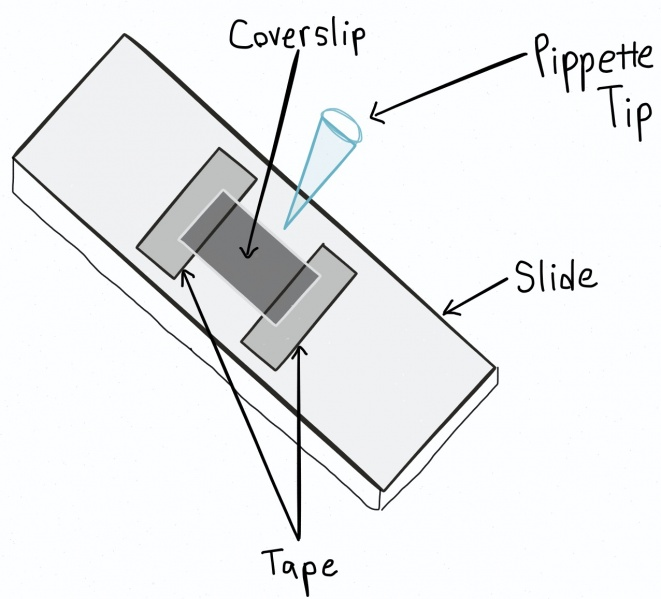
\includegraphics[width=0.5\linewidth]{images/OTZSlide.jpg}}
    \caption{Microscope slide assembly}
    \label{fig:OTZSlide}
\end{figure}

\begin{enumerate}
    \item Place a Kimwipe on the table to the left of the trap to create a clean place to set the slide. Any dirt or oil from your finger can obscure the light and/or scatter the laser beam, polluting the results of your measurement. Hence, keeping the center of the slide clean and the cover slip clean are important. Take out a microscope slide and place it on the clean surface.

    \item Create a ``channel'' about half as wide as a coverslip by placing two thin pieces of double-sided tape (use scissors) on the slide as shown in the diagram. Do not make the tape slices too wide or the slide will rest unevenly in the slots on the microscope stage.

    \item Place a coverslip directly over the gap between the two double sided tape strips. Use the small, square coverslips, not the rectangular ones (as is shown in the figure). The width of the coverslip will be smaller than the width of the slide, that is ok. Just center the cover slip over the two pieces of tape and the slide. Use the end of a pipetter to gently press the coverslip against both pieces of tape. The tape should hold the coverslip firmly in place.

    \item After shaking your sample solution in the vial and placing your slide assembly coverslip up, pipette $\sim$10-15 $\mu$L onto one of the protruding sides of the slide. The channel will suck the fluid under the slide and fill the gap. You could, of course, put the sample in first but if you put too much, the coverslip will force some of it on top of the tape and weaken the bond. The former method prevents the coverslip from sliding around when it is in place over the objective.

    \item Lightly coat both ends of the channel with nail polish. This will seal the channel and delay the sample drying.

    \item To insert slide onto stage, see the ``Slide Loading'' section located below.
\end{enumerate}

\subsection{Microscope Operation}

\textbf{Illuminator}

Turn on the red LED by turning on the power supply on the shelf over the optical table. You should see a  red glow emitted from above the stage. Adjust the voltage knob to get a brighter or darker image. The current will slowly increase as voltage increases, but do not exceed 8.7V for voltage and 0.35A for current.

\textbf{Joystick}

\emph{\textbf{Make sure not to run or turn the pico-motors to their ends. They should be centered about their movement.}}

Turn on the power switch on the controller for pico-motors and the QPD located on the shelf above the optical table. To use the joystick, you need to select which motor drives which axis by pressing the ``set axis'' and ``motor'' buttons on the joystick. To set motor A to drive the x-axis and motor B to drive the y-axis, use the following button sequence:

\begin{enumerate}
    \item set axis

    \item motor

    \item set axis
\end{enumerate}

The button at the tip of the joystick doesn't serve a function in this lab.

After doing this, the red LED indicators at the top of the joystick should alternate between the two sets of three lights being illuminated. The first set is ``Set X'', ``Driver 1'', and ``Motor A''. The second set is ``Driver 1'', ``Set Y'', and ``Motor B.'' To check if you've set up the joystick correctly, you can check to make sure the following table is correct.

\textbf{Controlling Sample Movement. ``Stage Control Software'' refers to the large buttons in the Stage Control matlab program, and ``Image Movement'' refers to the way the image moves on the computer camera viewer.  All joystick operations are from the reference point of standing as if you were typing on the keyboard for the computer.}

\begin{center}
    \begin{tabular}{c|c|c|c}
        Joystick Direction & Software Control Button & Image Movement & Stage Movement \\\hline
        $\uparrow$    & Left  & Down  & Left (+y) \\\hline
        $\downarrow$  & Right & Up    & Right ($-$y) \\\hline
        $\rightarrow$ & Up    & Left  & Forward (+x) \\\hline
        $\rightarrow$ & Down  & Right & Backward ($-$x)
    \end{tabular}
\end{center}

\emph{If you ever accidentally hit one of the buttons the joystick will change operation modes.} To get back to the correct mode:

\newpage

\begin{enumerate}
    \item Click all three buttons simultaneously, all of the red LEDs should be lit.

    \item Wait until some of the LEDs turn off

    \item Click Set Axis, Motor, Set Axis
\end{enumerate}

\textbf{Slide Loading}

\begin{enumerate}
    \item Lower the objective lens using the micrometer adjustment/positioning knob (turn it clockwise as viewed from above) so that the lens will not be scratched (or even touched) by the microscope slide as it is being loaded. Lower it all the way--this will take quite a few turns.

    \item Place a tiny drop of the immersion oil on the lens using the dip stick in the bottle of oil. Let the oil run off of the dip stick back into the bottle for 10 sec before proceeding. Avoid touching the dip stick to the glass in the center of the objective. \emph{Oil only needs to be added to the objective about every other slide.} (Note: if immersion oil doesn't fill the gap between objective and coverslip, air bubbles will prevent stable trapping or deflect the beam off the center of the QPD.)

    \item \emph{Place the slide into the slot on the stage with the cover slip} \textbf{down}. (This is an inverted microscope.)

    \item Raise the objective by turning the positioning knob counterclockwise until you see the oil make contact with the cover slip. Make sure there are no air bubbles in the immersion oil or in the chamber where the light passes through. You'll continue to adjust the objective height to focus on the specimen, below.
\end{enumerate}

\textbf{Viewing the specimen}

\begin{enumerate}
    \item Start the optical trapping program and use the Camera View push button to turn on the camera. The live video image should then be visible in the FireView window.

    \item With the trapping laser on and the emission filter off (in the run wheel), move the objective up and down to find the reflection of the laser on the coverslip and slide (i.e. you will see two spots as you move the micrometer knob up and down, one is from the reflection of the laser off of the coverslip, and the other is off of the slide). The slide reflection is much more symmetric. Focus again on the coverslip, and search for beads floating above it. Keep track of the position of the objective relative to the coverslip. The lens should never be so low that immersion oil fails to fill the gap, nor so high that it pushes the slide up off the stage. If beads are scarce, you may need to move the stage horizontally with the joystick to find some.

    \begin{enumerate}
        \item As you adjust the objective lens with the micrometer positioning knob, you will see the laser beam focus on the camera viewer at two different heights of the objective lens. You will be able to view the beads being trapped when the objective lens is positioned near these two heights. The beads should be in focus, and moving around. If they are all stationary, the beads may have sunk to the bottom and you will need to prepare a new slide.

    \end{enumerate}

    \item Adjust the LED voltage and camera shutter speed as needed to get a good image. Keep in mind that a higher LED voltage will allow for a faster shutter speed and frame rate.

    \item Once the slide is loaded into the slots on the stage, do not make any adjustments to the slide. The slide should sit all the way in the grooves and should not ``teeter'' about the objective. All adjustments from here will be made using the joystick.
\end{enumerate}


\begin{figure}[h]
    \centering
    \href{http://experimentationlab.berkeley.edu/sites/default/files/OTZ/Beads.png}{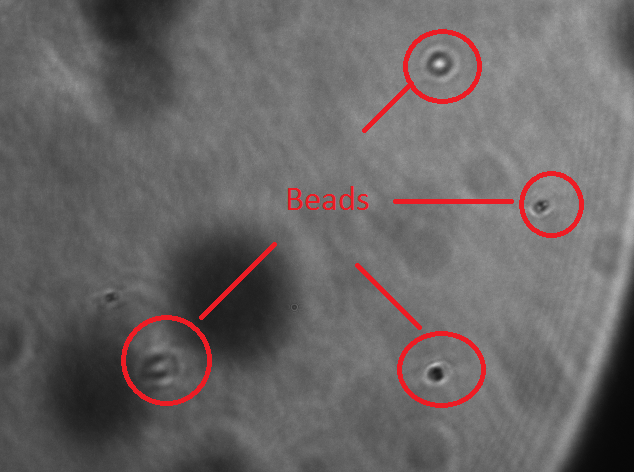
\includegraphics[width=0.7\linewidth]{images/Beads.png}}
    \caption{This is an example of what you should be seeing in your camera. The circled spots are the 1.01 micro meter silica beads.}
    \label{fig:Beads}
\end{figure}

\textbf{After you are finished}

When you are done trapping and collecting data (see below) power down everything and remove the slide from the stage. Be sure to lower the objective lens before removing the slide by turning the positioning knob clockwise.  Dispose of slides in the glass disposal box out in the lab. Dispose of pipette tips and kimwipes in the regular trash.

\subsection{Trapping Laser operation}

\textbf{Temperature Control} The SRS LDC501 controller for the trapping laser is on the shelf above the table. The unit contains both a Temperature Controller (TEC) and the Laser Diode Control. It is important to make sure that both parts of the controller are configured and set correctly. Begin by configuring the temperature sensor:

\begin{enumerate}
    \item Turn on the unit (by turning the key to the right), and turn on the TEC Control. Make sure the TEC is in CT mode. Press ``Config'' and arrow up until the ``TE Cfg: Sensor'' menu is illuminated. Use the wheel to scroll down to ``*3) NTC auto'' and press Enter.

    \item Press the down arrow key to move to the ``TE Cfg: Model'' page. Scroll to ``*0) NTC B,R(t),t'' (if it is not already on it). Arrow down to set the values of Β, R($t_0$), and $t_0$, which should be 3800C, 10k$\Omega$, and 25C, respectively.

    \item Room temperature should read on the ``Thermoelectric Cooler'' display.

    \item Press the ``Set'' key. Arrow all the way up, and set T to 25C.

    \item By arrowing down to the next item, set ``TEC Ilim'' (Current limit) to 1.4A, ``Tmax'' to 50C, Tmin to 0C, and ``TE Vmin'' to 8.00V.

    \item Press ``Config'' again and arrow down to ``PID vals.'' Enter the following settings for the P, I, and D loop gain parameters: P = $-$0.50A/C, I = 0.360/s, D = 0.65s. Also enter the settings: tunestep = 0.140A, CC $\leftrightarrow$ CT lock when on: *N, and the trip-off settings: TEIlim: *N, TE Vlim: *Y, Tmax: *Y, Tmin: *Y, SenseFault: *Y.
\end{enumerate}

Many, if not all, of these settings, and the ones for the laser control, are likely already set to what they should be. If this is the case, then great. \textbf{It is important to make sure the proper settings are used}.

\newpage

The TEC has a preset current limit, $I_\text{LIM}$, of 1.4 A and the resistance, $T_\text{ACT}$, should be around 10.0 k$\Omega$, and always within the range 9.5 to 10.5 k$\Omega$. This should already be set, but it is important to make sure it is not changed. The TEC, when set properly and turned on, will control the temperature of the laser diode , which prevents temperature-related power fluctuations. It should not need to be adjusted.

\textbf{Laser Diode Control} Control of the laser diode power is via the Laser Diode Control. Once the TEC has been set and turned on, the LDC can be used.

\begin{enumerate}
    \item Turn on the power for the Laser Diode Control. Make sure it is in CC mode.

    \item Press ``Config,'' and set the following settings in the same way as was done for the TEC. IRange: *1)500mA, CC BW: *1) high 1.2 MHz, Modulate: *N.

    \item Press ``Set.'' Arrow down to ``Ilim,'' and set the value to 500mA. Arrow down twice to ``LD Vlim,'' and set the value to 2.3V. Arrow back up to ``LD I'' and set the operating current value to 490.00mA. The maximum current limit has been set to 500.00 mA, but the actual operating current has been set to 490.00mA.
\end{enumerate}

\subsection{QPD Centering}

\emph{\textbf{Note: Do not over turn the QPD adjustment knobs, you will damage the mount and not be able to adjust the QPD to the center position.}}

Before taking data from the QPD, the QPD should be aligned so that the laser hits it in the center, resulting in voltages $V_x$ and $V_y$ being zero. Once you have opened the program, have turned on the LED and QPD, and have trapped a bead, you can zero the QPD signal in the QPD readout window. (Note: If you center the QPD before trapping a bead, the QPD readouts will not be zeroed after trapping a bead.)

The QPD signal is indicated by the blue ``x'' on the $V_y$ vs. $V_x$ graph. If this is not centered at the origin, adjust the knurled adjusting screws on the top and front of the QPD mount to bring the blue ``x'' to the origin.

If you are unable to zero the signal, first check to see if something like a second bead or debris has entered the trap (e.g. disable the laser and watch how many beads leave the trap). Also check that the green fluorescent laser is off whenever analyzing QPD readouts, as this laser affects the results.

The QPD zero signal will vary somewhat with the power level of the laser. Hint: If you are doing calibrations with beads at multiple power levels, you can zero the QPD signal at the highest power level, and then switch to lower and lower power levels without too much problem. If you precisely zero it at a low power level, you will find more drift in $V_x$ and $V_y$ as you move to higher power levels.

\subsection{Trapping Procedure}

\textbf{BE PATIENT IN FOCUSING THE MICROSCOPE. This experiment was tested and verified to be working on 09/30/2015}

\begin{enumerate}
    \item To get familiar with the location of the laser trap vertically with respect to the slide and coverslip and horizontally with respect to the camera's field of view, look for reflections of the infrared beam off of the slide and coverslip. These will look like focused beams in the camera viewer. To do this, find a place on the slide with no beads or cells nearby and turn on the laser at a medium power level (set LD I to 300 mA). Make sure that the emission filter in the filter wheel is not in the light path, as it screens out all of the infrared. As you move the objective up and down, you will see a reflection of the laser off the coverslip and off the slide when each is in focus.
    
    \newpage

    \item To trap a bead, you can search with the laser on or turned down or disabled until you find one to trap. It is easiest to turn off the laser entirely while noting the trap's location in the camera viewer field of view. Then, using the objective adjustment knob, focus on a bead to trap. Using stage control, move this bead approximately to the location of the trap, and turn back on the laser. The laser will likely no longer be a focused spot as it was when it was reflecting off of the coverslip/slide. Instead you might see a diffraction pattern. This is ok, the trap is still there. You should see the bead fall into place in the trap. Silica beads tend to sink rapidly to the bottom of the chamber formed by the slide and coverslip, meaning that they will be sitting on the coverslip. If beads are dense, then look for one that is isolated from others before turning the laser power up.

    \item Once a bead is trapped, it will appear slightly unfocused because the equilibrium position of the trapped bead is generally slightly above the optical focus of the lens. As you move the slide with the joystick, the bead should remain fixed by the trap while the other contents of the slide move by. Theoretically, you should able to move the bead up and down by moving the objective up and down. This is difficult in practice however, as it is very easy to bump the microscope and knock the bead out of the trap. If the bead goes out of focus when you lower the objective, then the bead is stuck to the coverslip and not really trapped, so try another bead.

    \item To take QPD data from a free bead or other trapped object, move the bead above the coverslip about 3 $\mu$m (the finest gradations on the micrometer screw of the objective lens correspond to 1 $\mu$m of vertical travel) so that its motion will not be influenced by the wall effect. Think about why adjusting the micrometer screw affects the vertical position of the trapped bead, and \emph{be sure to explain this in your lab report.}

    \item Center the QPD (i.e. adjust the position of the QPD mount until $V_x$ and $V_y$ are zero).

    \item As you collect data, keep an eye on the bead to make sure that another bead does not get sucked into the trap. This is a problem especially with dense suspensions and higher power levels. When you finish with a bead, it is wise to release it and check the image to see if another bead was hiding below it in the trap.
\end{enumerate}

\begin{itemize}
    \item \emph{Experiment with trapping multiple beads at once to see if you can tell from the camera what is going on. How many can you trap at once?}

    \item \emph{How low can you turn the laser power before a bead escapes the trap? How does the behavior of the bead change at lower power?}
\end{itemize}

\begin{figure}[h]
    \centering
    \href{http://experimentationlab.berkeley.edu/sites/default/files/OTZ/laserwithbead.png}{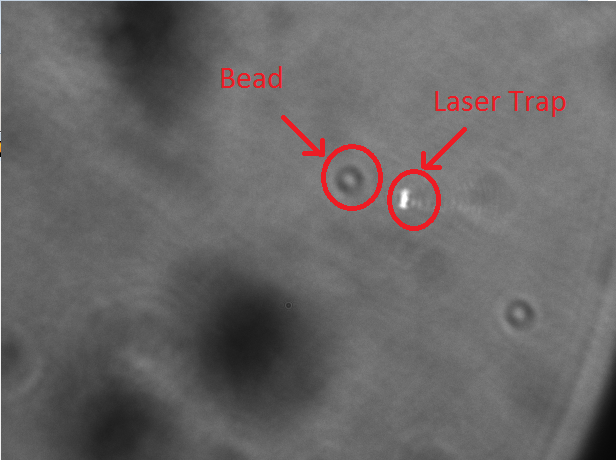
\includegraphics[width=0.5\linewidth]{images/laserwithbead.png}}
    \caption{This is an image of the laser trap approaching the silica bead.}
    \label{fig:laserwithbead}
\end{figure}

\begin{figure}[h]
    \centering
    \href{http://experimentationlab.berkeley.edu/sites/default/files/OTZ/trapped.png}{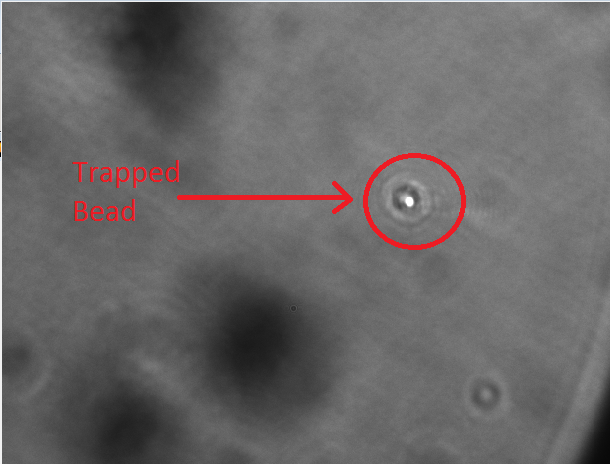
\includegraphics[width=0.5\linewidth]{images/trapped.png}}
    \caption{This is an image of a trapped silica bead.}
    \label{fig:trapped}
\end{figure}

\emph{If you are having trouble trapping beads you can try this alternative method}:

\begin{enumerate}
    \item Turn on the laser and note the lateral location of the trap in the camera viewer

    \item Turn off the laser and focus on a bead or several beads by adjusting the height of the objective

    \item Turn back on the laser \textbf{and} put the emission filter (in the wheel) in the beam path. This will block the infrared laser

    \item Using the joystick scan beads into the location of the trap (which you can no longer see because the emission filter is in place) and you should see the fall into the trap.

    \item This method might be easier because you might see a diffraction pattern of the laser when trying to focus on beads, which makes it difficult to see the beads.
\end{enumerate}

\subsection{Useful Matlab Code}

Before you begin taking and analyzing data, it is useful to learn how to programmatically load data from file. The obvious approach that many students take is to manually load each data set from its respective text file, but there are much more efficient ways of performing this task. For this experiment in particular, there will be two types of data files to handle. The first type is simply a text file with several columns of data, which can be accessed with the code below:

\begin{verbatim}
    fmt = repmat('\%f', 1, numberOfColumns);

    fid = fopen(file);

    datacell = textscan(fid, fmt, 'Delimiter', '\t', 'CollectOutput', 1);

    fclose(fid);

    Data = datacell{1};
\end{verbatim}

The data can now be retrieved from the Data matrix. This code will work for both the voltage and PSD data, assuming the numberOfColumns is correct. The second type of file is the \emph{Settings} text file, in which the information is organized into fields. By using the code below, you can retrieve the value of each field from the single-column matrix Settings:

\begin{verbatim}
    fid = fopen(file);

    Settings = fscanf(fid,'Sample Rate: %f\nNumberOfSeconds: %f\nParticleDiameter: %f\n
                      Viscosity: %f\nxStiffness: %f\nyStiffness: %f\nxSensitivity: %f\n
                      ySensitivity: %f\n');
    
    fclose(fid);
\end{verbatim}

Ideally, you will now be able to work much of the analysis required in this experiment into several Matlab scripts, while still retaining an understanding of the processes involved in the analysis.

\textbf{This is a Checkpoint: Call over a GSI or Professor and show them that you have successfully focused an image of the silica solution and that you are properly trapping a single bead. Also show that you have centered the QPD around zero on the graph display.}

\section{Part I. Calibration of the Optical Trap}

Observing specimens and trapping small objects is straightforward with the procedures described above. But to tap the full potential of the laser tweezers to precisely quantify size, position, and forces at nanometer and piconewton scales requires careful calibration. To save time, we are providing you with calibrations of the microscope image scale and the step-size of stage movements by the picomotors. We leave to you the more interesting calibrations, including translating the voltage measurements from the QPD into the position of the trapped particle relative to the center of the trap (QPD position calibration) and the force exerted by the trap on the particle (trap stiffness calibration). There are multiple techniques used to calibrate traps, and we'll let you try a few of them and compare their results and appropriateness.

\subsection{Microscope and Stage Calibration}

Results of these calibrations are provided below for your use. If you would like to perform them as part of your lab exercise, that is an option you may choose and we might substitute your results in the future.

\textbf{Pixel to meter conversion of the microscope image}

A micrometer slide with markings at 10 micron increments was used to measure the pixels/micron of the video image. The result: $1\mu = 27.17 \pm 1.5$ pixels (last measured by Eric Parsonnet, June 2015). If you want to use images captured from the video camera to analyze movements or sizes of structures, this information may come in handy.

\begin{figure}[h]
    \centering
    \href{http://experimentationlab.berkeley.edu/sites/default/files/images/400px-Stepsize-ayars.jpg}{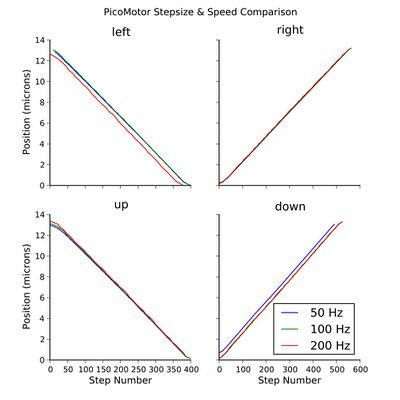
\includegraphics[width=0.5\linewidth]{images/400px-Stepsize-ayars.jpg}}
    \caption{Position v. Step Number}
    \label{fig:400px-Stepsize-ayars}
\end{figure}

\textbf{Stage picomotor step size}

The nominal step size given in the specs of these picomotors is 30nm and ideally would not vary with motors or between directions for one motor. However, the motors have to work against various springs in the X- and Y- stages, so the resistance to motion left and right (X) varies, as does resistance forwards and backwards (Y). In addition, the first few steps may vary in size as the stage starts up.

To find the average step size of motorized stage movements in +Y,-Y,+X,-X directions, beads were caused to stick to a microscope slide (see technique under position calibration below) and the slide was moved in each direction at a controlled rate with the picomotors. The particle tracking feature of the optical trapping software was used to record trajectories of several beads as they were moved by the stage with the laser off. The position of a bead was plotted vs. step number for 3 different frequencies of motor operation, as shown in the accompanying graphs. Step size was found to be pretty consistent for one direction after the first few steps, and step frequency did not seem to matter from 100 to 225 Hz. This calibration was last performed by Eric Parsonnet in June, 2015.

The average step sizes were:
\begin{align*}
    &\emph{left: } 37.04 \;\mu/\text{step} \\
    &\emph{right: } 27.78 \;\mu/\text{step} \\
    &\emph{up: } 25.64 \;\mu/\text{step} \\
    &\emph{down: } 35.71 \;\mu/\text{step}
\end{align*}
Using the Stage Control program provided within OTKBv7 (the MatLab GUI) we can find the speed for the different movements, given some set frequency. The speed can be determined by taking the distance per step (listed above) and multiplying by the frequency. This method was tested by Eric Parsonnet in June 2015, and was found to be correct.
\begin{align*}
    &\emph{left expected: } \left(\frac{\text{distance} = 37.04 \text{nm}}{\text{step}}\right)(\text{frequency} = 250)=\frac{9.26 \mu}{\text{sec}} \\
    &\emph{left observed: } 9.709 \pm .700 \frac{\mu}{\text{sec}} \text{ (expected is within error)}
\end{align*}
The others were checked as well, but it is not necessary for me to include them here. Long story short, if you need speed, use the stage control program to ensure consistency, take the above distances/step and multiply by the frequency of your scan to get speed.

\textbf{Note}: The directions above (left, right, up, down) refer to the apparent movements of the stage according to the camera image, e.g. when a stuck bead appears to be moving to the right in the video, we call that ``right.'' One complication introduced by the fact that the camera looks at the slide from underneath is that left and right are reversed from our perspective looking down at the slide. Up and down are not reversed, meaning that up indicates movement of the slide away from you and down is towards you. To avoid confusion, we use the directions apparent from the camera image.

\subsection{Position and Stiffness Calibration of the QPD}

\newpage

Calibration of the QPD's response to movements of the trapped objects typically use microspheres because of their symmetry and standardized characteristics, such as refractive index, size, shape, etc. In some cases, calibration is performed with a bead that is similar in size and shape to the biological specimen of interest. In others, the bead itself is used in an experiment to apply forces to the biological specimen. For example, a bead can be attached to one end of a macromolecule such as DNA as a handle to pull on. If the other end of the molecule is stuck to a coverslip or a pipette, the bead can be moved by the trap to apply precise forces to the molecule or other structure. In this lab you can do your calibration with Silica beads of 1 or 2 micron diameter, and should plan to use the same bead size for all of your calibration techniques.

\textbf{What is Position Calibration?} Within a narrow range around the trap (about 100-200 nm), the voltages $V_x$ and $V_y$ from the QPD are linearly related \cite{Gittes} to the distance of the bead from the center of the trap along each axis. The position calibration, also called \emph{sensitivity}, allows us to translate our raw $V_x$ and $V_y$ data into distance data. Sensitivity, $\rho$, is usually given in units of Volts/$\mu$. Of course, the power setting of the laser will affect the light intensity incident on the QPD, and thus the voltage responses, so rather than a single conversion we really want the relationship between sensitivity and laser power. This normally is fairly linear, so measuring sensitivity at 4 power levels is plenty to characterize the relationship.

We have two independent methods for performing position calibrations. The first, called the \textbf{stuck bead scanning method}, is to move a bead stuck to a slide through the center of the trap at a controlled speed with the motorized stage and record the $V_x$ or $V_y$. In the linear region near the center of the trap, the slope of $V_x$ vs. distance is the inverse of sensitivity. The second method, less direct, is to apply our understanding of the physics of Brownian motion of a bead of known size in a medium (water) of known viscosity. By trapping a free bead and recording $V_x$ and $V_y$ at high frequency, a Power Spectrum Density (PSD) can be calculated to give an estimate of sensitivity. We'll call this the \textbf{PSD method}. Try both of these methods as detailed below and see how comparable are the results.

\textbf{What is Stiffness Calibration?} Forces in optical traps generally cannot be measured directly. Rather, the force on a trapped particle is calculated by multiplying the displacement of the particle from the trap's center by the stiffness of the trap. That is, the trap obeys Hooke's law, $F = -k x$, where `$k$' is the stiffness of the trap.

\begin{center}
    \begin{tabular}{l|l|l}
        Method/how to sample & Position & Stiffness \\\hline
        \textbf{1. Stuck Bead:} sample 8s@1 kHz & X & \\\hline
        \textbf{2. PSD} (with free bead): sample 4/3 s@12kHz & X & X \\\hline
        \textbf{3. Equipartition} (with free bead): sample 8s@1kHz, down-sample to 30 Hz & & X
    \end{tabular}
\end{center}

A variety of methods can be used to calculate trap stiffness, each with advantages and drawbacks. We'll use two in this lab, both exploiting the effect that the trap has on inhibiting Brownian motion of a trapped particle. The \textbf{Power Spectrum Method} uses the same data as for the position calibration method of that name. The second, called the \textbf{Equipartition Method}, analyzes the variance in position of the particle over a longer time period at much lower frequency. Compare the results of these two methods and consider which might be preferable in different applications.

To summarize, you will use three techniques for position and stiffness calibration, resulting in two position calibrations and two stiffness calibrations, as depicted in the accompanying table.

\subsubsection{Stuck Bead Scanning Method (Position Calibration)}

We recommend scanning a stuck bead along each orthogonal axis through the center of the trap, considering $V_x$ and $V_y$ independently of one another. A more complete calibration would require raster scanning back and forth in a grid to cover the entire active 2D region of sensor, but this is problematic due to some hysteresis and imprecision in our motorized stage so we'll stick to measurements along the axes.

\newpage

\textbf{Stuck Bead Sample Preparation} Exposing the beads to a salt solution causes them to stick to glass by hydrophobic interactions. A 1 M NaCl solution is provided for this purpose. You can simply substitute the salt solution for water, and again make a 1:10,000 dilution. Alternatively, you could combine the salt solution with a bead sample directly on a slide rather than making a separate vial. To do this, try adding 5 microliters of your previous 1:10,000 dilution of a bead stock in water to 30 microliters of 1 M NaCl on a slide. After adding a coverslip, invert the slide. It may take up to 10-20 min to get good adhesion, and some beads will stick better than others. You may need to adjust the bead concentration to get a reasonable density of beads on your slide.

\begin{figure}[h]
    \centering
    \href{http://experimentationlab.berkeley.edu/sites/default/files/images/StuckBead500.png}{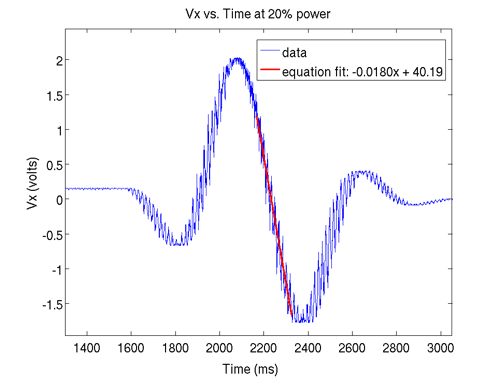
\includegraphics[width=0.7\linewidth]{images/StuckBead500.png}}
    \caption{A plot of $V_x$ vs time for a stuck bead moved from left to right. The red line is fitted to the data from the linear region.}
    \label{fig:StuckBead500}
\end{figure}

\textbf{Scanning Procedure}

\begin{enumerate}
    \item Center the QPD signal without a bead near the trap and with the laser at the highest power you will be using.

    \item Set a sample rate of 1kHz and history length of 8s (or however long you need to capture the data). You can ignore most of the other settings for now.

    \item Locate a bead that is firmly stuck, that is, it does not seem to ``wobble'' as it is dragged through the center of the trap.

    \item Focus the microscope so that the bead is at the same height that it would be if it were freely suspended but trapped. It should be a little out of focus. (Use your prior experience trapping beads to judge this.)

    \item Center the stuck bead in the laser trap, using the joystick. The QPD signal should read approximately $V_x$ = 0, $V_y$ = 0 and small motions along the X or Y axis should cause large changes in $V_x$ or $V_y$, respectively).

    \item Once the bead is centered, switch to software control of the stage and set the step number (preferably at least 100) and frequency (50-150 Hz) how you want.

    \item Move the bead away from the trap center in the -X direction (direction is arbitrary) by the set number of steps and stop the QPD readout.

    \item Set the stage control window to move the bead in the +X direction twice as far as you moved the bead in the -X direction.

    \item Click the Save Voltage Data and Graph button to save the data to file.

\end{enumerate}

This will take 8 seconds of QPD voltage data sampled at 1kHz and saved as a text file with name and location you specified. A graph of the QPD readout vs. time will be shown when you click the save button, and the graph itself will be saved along with your data. The graphs should both read roughly 0 at the very beginning and end of the run and you should see a signal like that of the one pictured above in the direction in which you are scanning the bead. The perpendicular direction (in our case, Y) should show very little change and be roughly symmetric around the center of the trap, as determined from the $V_x$ plot. If $V_y$ varies a lot, you might recenter the bead and try again. Keep in mind that there is some hysteresis in the motors/stage and sometimes the coverslip may be dragged a little by the viscosity of the immersion oil. Reducing the number of steps you go away from the center of the trap may help.

Repeat this measurement for the Y axis and then repeat both X and Y for each power level you choose for calibration.

Plot both $V_x$ and $V_y$ vs. index and zoom in to note the time points that bound the linear region that lies in the center of the trap. Perform a linear regression on this time range of data only and use the appropriate sample rate, step size, and frequency to calculate the sensitivity for this axis and power level.

\textbf{Using Matlab}

Once you have determined the start and end indices for the linear range of the stuck bead data, you can convert your x-axis units to $\mu$m using a few known quantities (hint: the x-axis is equivalent to milliseconds due to the sample rate used, and you can calculate the speed of the stage in $\mu$m/ms to make the conversion). Then, a linear regression can be performed on the linear region of the data using a first-degree polyfit function in Matlab. From this you can find the sensitivity of the trap in V/$\mu$m, and the linear range of the trap. Once you determine the trap stiffness below, you can calculate a crude estimate of the maximum trapping force of the trap. (Note: the stuck bead scanning technique tells you how wide the linear region of the position detection extends, and does not necessarily correspond with the linear region of the force produced by the trap. However, since we can only determine the force on a bead indirectly using trap stiffness and the distance from center, a departure from the linear region of position detection essentially results in a departure from the linear region of our calculated force.)

Once you have calculated the sensitivities for all four power levels in X and Y, plot them versus laser power in Matlab.


\textbf{This is a Checkpoint: Call over a GSI or Professor and show them the plot you have made of sensitivity vs laser power for X and Y. Explain how the sensitivities varies with power and what is happening.}

\subsubsection{Power Spectrum Method (Position and Stiffness)}

The thermal motion of a spherical bead of known size suspended in water is well characterized. As the laser power is turned up on a trapped bead, the Brownian motion of the bead is constrained more and more by the increasing trap force restoring the bead to the center of the trap. A statistical analysis of this motion allows us to estimate both the sensitivity of the trap and its stiffness.

\textbf{Procedure}

\newpage

\begin{enumerate}
    \item Starting with a slide loaded with a sparse suspension of beads in water, trap a bead and move it well away from other beads.

    \item With the emission filter on to remove the trapping laser reflection off the coverslip, lower the bead until it hits the coverslip and goes out of focus. Using the focus as a guide, find and record the height of the coverslip. The z-axis adjustment knob has micrometer marking, which you can use for this purpose.

    \item From the coverslip, raise the bead 20 -30  microns up (note that 1 revolution on the micrometer screw corresponds to 500 microns displacement). If the bead is too low, edge effects due to contact with the coverslip will restrict the brownian motion, while at heights above 20 -30 microns the optical trap loses its tight focus (the objective lens is designed to focus the laser through oil, so it will not focus well far above the coverslip)

    \item Record QPD data using the 'Save Voltage Data and Graph' button with the 'Sample Rate' set to 5,000 Hz and the 'History Length' set to 5 seconds. You can get an idea of what the fitted PSD data will look like, and what sensitivity/stiffness values you should roughly get, by clicking 'Fit PSD and Save Data/Graph'. However, you will have to do the fit yourself as well starting from the voltage data, since the OTKBv7 program's fit will not supply you with all the necessary information.

    \item Repeat data collection at each of the laser power settings you have chosen for your calibration. (If you have centered the QPD at the highest power setting, you shouldn't have to recenter between power settings.)

    \item Collect voltage data for at least two beads.

\end{enumerate}

The PSD Method stiffness measurement requires knowledge of the hydrodynamic drag on the particle. For a sphere, the Stoke's drag relation is well known, and requires knowing the diameter of the bead and viscosity of the fluid. The Stoke's relationship is not valid close to a wall, so a particle must not be near the surface of a slide or coverslip.

The Power Spectral Density (PSD) \cite{Reif} of a trapped bead has a Lorentzian profile described by:
\begin{equation}
    S_{\nu\nu} = \frac{\rho^2 k_b T}{\pi^2 \beta(f_o^2+f^2)}
\end{equation}
in Volts$^2$ / Hertz. Where $\beta = 3\pi\eta d$ is the drag, $\eta$ is the fluid viscosity of water, $d$ is the diameter of the bead, $\rho$ is the sensitivity of the trap, and $f$ is the frequency of bead vibrations. If the fluid is water then we can take: $\eta = 8.90 \times 10^{-4}$ Pa*s. Using this, a curve can be fit to the log of the data sets giving the rolloff frequency $f_o$. In addition the rolloff frequency relates to the relaxation time: $\tau_o = 1/2\pi f_o$.

\emph{Using Matlab}

(\textbf{All Matlab .m files can be found zipped  \href{http://experimentationlab.berkeley.edu/sites/default/files/ZIP\_files/OTZ\_Matlab\_files.zip}{here}.})

Several Matlab programs are provided, including: (\textbf{All Matlab .m files can be found zipped  \href{http://experimentationlab.berkeley.edu/sites/default/files/ZIP\_files/OTZ\_Matlab\_files.zip}{here}.})

\href{http://experimentationlab.berkeley.edu/sites/default/files/matlab\_fitting/FitlogcurvevarXV2.m}{\textbf{FitlogcurvevarXV2.m}}

\href{http://experimentationlab.berkeley.edu/sites/default/files/matlab\_fitting/FitlogcurvevarYV2.m}{\textbf{FitlogcurvevarYV2.m}}

One useful analytic method for this part of the lab minimizes the least-squares distance of every point from the predicted curve, giving two parameters of the equation, alpha and $f_o$. The Lorentzian can be recast as the equation: $\log{S_{\nu\nu}(f)} = \log{\alpha} - \log{(f_o^2+f^2)}$.

To use Matlab, you will have to import your data from the text files into the workspace. These text files will have two columns - one for X voltage and one for Y voltage - and can be imported into Matlab easily with the aid of the ``Useful Matlab Code'' section above. It is best if you use a matlab script to perform these and the following tasks, rather than do everything in the command window.

Once the data is imported, you will need to convert it to Power Spectral Density data using the built-in Matlab function ``pwelch.'' It is recommended that you look up what this function does, and look in the ``OTKBv7'' code to see its correct usage. Once you have done this, you can represent the data with a three column matrix: frequency, x-direction PSD data, and y-direction PSD data. You can then call the functions \emph{fitlogcurvevarX} and \emph{fitlogcurvevarY} within this script. These functions will allow you to input as many three-column data sets at once as you wish. They use a non-linear fitting procedure to fit the theoretical curve to log transformed data, returning alpha (a\_x or a\_y) and rolloff frequencies (fo\_x or fo\_y). The plot(s) from the functions relate log(PSD) vs. log(freq), and should look like the Power Spectrum Density as it appears in the QPD readout window.
\begin{verbatim}
    [a_x fo_x] = fitlogcurvevarX( data1, pwr1, data2, pwr2, ... )
\end{verbatim}
Then, using properties of logarithms and the two Lorentzian equations above, it should be possible to solve for x and y sensitivities from the alpha values a\_x and a\_y.

Similarly, the rolloff frequency parameters found from \emph{fitlogcurvevarX} and \emph{fitlogcurvevarY} give the trap stiffnesses from the following relation:
\[
    k = 2 \pi f_o \beta
\]
again where $\beta$ = $3\pi\eta d$  is the drag, $\eta = 8.90 \times 10^{-4}$ Pa*s is the viscosity of water, and $d$ is the diameter of the bead (in meters).

Finally, you will want to graph $\rho_x$, $\rho_y$, $k_x$, and $k_x$ versus laser power, and fit a line to each of them to determine their dependence on laser power. You may consider averaging the values you obtained from each bead first.


\textbf{This is a Checkpoint: Call over a GSI or Professor and show them your graphs of $\rho_x$ , $\rho_y$, $k_x$, $k_y$ versus laser power as well as your solutions for $x$ and $y$ sensitivities from the alpha values $a_x, a_y$.}

\subsubsection{Equipartition Method (for Stiffness)}

This method is based on the equipartition theorem, which states that each degree of freedom in a harmonic potential has $\frac{1}{2}k_bT $ of energy. Using this theory, we can relate the thermal energy of a system to the instantaneous displacement of small particles via the statistical mechanical idea of heat as: $  \frac{1}{2}k_b T = \frac{1}{2}k_x \langle(x-\langle x\rangle)^2\rangle $, where $\langle x\rangle $ denotes the average over $x$, the position of the particle along the x direction. Since $\langle(x-\langle x\rangle)^2\rangle $ is the variance of $x$, stiffness can simply be calculated from the variance of the bead position at each power level.

This method has a few requirements you should be aware of.

\begin{enumerate}
    \item The variance used must be of particle position (distance from the center of the trap in x or y), not of the voltage from the QPD. So you need to use the position calibration (sensitivity) to convert $V_x$ to $x$ before taking the variance. You can try using sensitivities from the Stuck Bead and PSD methods, and you may find that this choice has a big effect on the stiffness values you obtain.

    \item The observations used in this analysis are assumed to be independent of one another. Hence, the particle positions must be taken at intervals greater than the relaxation time, $\gg \tau_o$, which can be derived from the rolloff frequency of the trap as described in the ``PSD Method'' section. The program will not allow you to set the Sample Rate this low, so it may be simpler to use the data taken for the PSD method and down-sample it in Matlab.

\end{enumerate}

\emph{Using Matlab } (\textbf{All Matlab .m files can be found zipped }\href{http://experimentationlab.berkeley.edu/sites/default/files/ZIP\_files/OTZ\_Matlab\_files.zip}{\textbf{here.}})

Here we will use the program \href{http://experimentationlab.berkeley.edu/sites/default/files/matlab\_fitting/Equipartition.m}{\textbf{Equipartition.m}} . After inputting the values for sensitivity at each power in both the x and y-directions, as well as the data sets with their corresponding power levels, it will graph and calculate stiffnesses in both X and Y and perform a linear fit. A quick glance at the program in the Matlab editor should be sufficient to understand how it operates.
\begin{verbatim}
    [Kx,Ky] = equipartition(x_sensvspwr, y_sensvspwr, data1, pwr1, data2, pwr2, ...)
\end{verbatim}
\textbf{This is a Checkpoint: Call over a GSI or Professor, show them your values for stiffness and discuss your answers to the following questions:}
\begin{itemize}
    \item \emph{Why might there be a difference in $k_x$ and $k_y$}?

    \item \emph{How do the assumptions of the PSD method and Equipartition method for measuring stiffness differ?}

    \item \emph{Why must the successive data points be independent?}

    \item \emph{How does this idea of autocorrelation between successive values of the position, $x$, relate to the Power Spectrum Density?}

    \item \textbf{BONUS:} \emph{How can this independence be tested? i.e. How can the correlation be measured?}

    \begin{itemize}
        \item To understand how to test this it may help to consult \cite{Reif} and look into the ideas of \textbf{covariance} and \textbf{autocorrelation}, also found in the same \href{http://physics111.lib.berkeley.edu/Physics111/Reprints/OTZ/biowikipedia.pdf}{\textbf{definitions sheet}}. If time permits and you are interested in this idea, by taking several data sets (maybe 100 of 1 second each), each giving a value: $k_i$, you should see some variance in $k$. You can measure the mean and standard deviation in $k$ using 2 different sampling rates (one above and one below the correlation time of the trap) and then measure the autocorrelation.
    \end{itemize}

\end{itemize}

\section{Part II. Investigating Flagellar Locomotion in E. Coli}

As defined in the \href{http://physics111.lib.berkeley.edu/Physics111/Reprints/OTZ/biowikipedia.pdf}{\textbf{definitions sheet}} and again on wikipedia (no guarantee of accuracy there) \emph{\href{http://en.wikipedia.org/wiki/Escherichia\_coli}{\textbf{Escherichia coli}}} (abbreviated \emph{E. coli}) is a rod-shaped bacterium about 1 $\mu$m in diameter by 2-4 $\mu$m long. It normally occurs in the intestines of humans and all warm-blooded animals. Most strains, including the one we will study, are harmless to humans. \emph{E. coli} has a bad reputation due to some pathogenic strains that produce dangerous toxins causing diarrhea and some other diseases.

\begin{figure}[h]
    \centering
    \href{http://experimentationlab.berkeley.edu/sites/default/files/images/400px-Ecoli800.jpg}{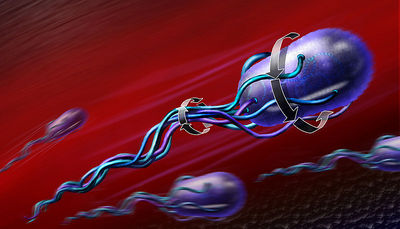
\includegraphics[width=0.5\linewidth]{images/400px-Ecoli800.jpg}}
    \caption{An artist's depiction of \emph{E. coli} in a run showing how the flagellar filaments intertwine to form the flagellum. Note that rotation of the flagellum is in the same direction as rotation of the individual filaments, while the cell rotates in the opposite direction. \emph{Credit:} Nicolle Rager Fuller/National Science Foundation.}
    \label{fig:400px-Ecoli800}
\end{figure}

\emph{E. coli} is propelled in liquids by a set of four or more helical flagellar filaments that arise from separate positions on the cell surface but intertwine to appear as a single flagellum in forward movement. A cell may lose its flagella under some conditions, and regenerate them under others. Although motile cells on a crowded slide may appear to be moving pretty randomly, a cell actually can modulate its swimming to follow gradients of chemicals, temperature, or light. It accomplishes this by varying the ratio of two swimming behaviors. The first, called a ``\textbf{run}'', is swimming forward in a steady, mostly straight path. The second behavior, called a ``\textbf{tumble}'', is an erratic motion that causes the next run to be in a new direction, pretty much at random. If the cell senses that the environmental gradient is getting worse as it swims, then a tumbles are more frequent; if it is getting better, tumbles are less frequent. So motility of the cell is facultative and under at least crude directional control.

\newpage

The running and tumbling behaviors are caused by a simple switching of direction of motors. Each flagellar filament is driven by a rotary motor at its base that turns counterclockwise (CCW) in forward swimming, as all the filaments intertwine together. During running, the cell swims steadily forward in a direction parallel to the long axis of the cell with the flagellum pushing. Tumbling occurs when one or more of the flagellar filaments turns clockwise (CW), causing the flagellar filaments to separate and beat erratically. You can see the run and tumble pattern behavior in a series of \href{http://www.rowland.harvard.edu/labs/bacteria/movies/ecoli.php}{\textbf{movies}} depicting fluorescently labelled \emph{E. coli}.

Alternatively, the videos are listed below:

\begin{itemize}
        \item \href{http://physics111.lib.berkeley.edu/Physics111/Reprints/OTZ/cellsnearslide.avi}{\textbf{cells near slide}}

        \item \href{http://physics111.lib.berkeley.edu/Physics111/Reprints/OTZ/curlybundle.avi}{\textbf{curly bundle}}

        \item \href{http://physics111.lib.berkeley.edu/Physics111/Reprints/OTZ/cytoplasmicstreaming.avi}{\textbf{cytoplasmic streaming}}

        \item \href{http://physics111.lib.berkeley.edu/Physics111/Reprints/OTZ/filamentleavingbundle.avi}{\textbf{filament leaving bundle}}
        
        \item \href{http://physics111.lib.berkeley.edu/Physics111/Reprints/OTZ/filamentsonstuckcell.avi}{\textbf{filaments on stuck cell}}

        \item \href{http://physics111.lib.berkeley.edu/Physics111/Reprints/OTZ/fluorescentbundlesslow.avi}{\textbf{filaments on stuck cell, \emph{slowed}}}

        \item \href{http://physics111.lib.berkeley.edu/Physics111/Reprints/OTZ/semicoiledbundle.avi}{\textbf{semi-coiled bundle}}

\end{itemize}

With the optical trap, you can trap individual cells, characterize the running and tumbling motions from the QPD signal, and investigate some aspects of the motion.

\subsection{Planning Your Investigation}

Begin by reading carefully the following two papers on using optical traps to study swimming in \emph{E. coli},

\begin{itemize}
    \item S. Chattopadhyay, R. Moldovan, C. Yeung, X. L. Wu, Swimming efficiency of bacterium Escherichia coli. \href{http://physics111.lib.berkeley.edu/Physics111/Reprints/OTZ/swimmingefficiency.pdf}{\textbf{Proc. Natl. Acad. Sci. (2006)}}. Uses optical trap similar to ours; good intro to E. coli locomotion and ideas for experiments.

    \item T. L. Min, P. J. Mears, L. M. Chubiz, C. V. Rao, I. Golding, Y. R. Chemla, High-resolution, long-term characterization of bacterial motility using optical tweezers, \href{http://physics111.lib.berkeley.edu/Physics111/Reprints/OTZ/bacterialmotility.pdf}{\textbf{Nature Methods (2009)}}. Note that following the reference section of the paper there is a supplemental online methods section, which contains links to a separate pdf of supplemental figures. This study features excellent experimental work on \emph{E. coli} swimming using a setup that generates two traps with a single laser beam, allowing better control over the orientation of the cell.
\end{itemize}

Consider what kinds of patterns you might expect in your data on trapped cells and what questions you might be able to investigate.

Some suggestions you might try:

\begin{enumerate}
    \item How fast do cells rotate during a run? Is it consistent for one cell? Does it vary with the power of the laser?

    \item What is the pattern of running and tumbling? How frequently is a run interrupted by a tumble?

    \item Does reversal of the cell direction ever occur while the cell is trapped? (Reversal would occur by the flagella reorienting to the other end of the cell rather than the cell turning abound.)

    \item What is the distribution of cell swimming speeds? (You can use the particle tracker feature on the video camera images to measure this without using the trapping laser.)

    \item What is the propulsive force required to offset hydrodynamic drag? The Stoke's Drag for laminar flow past a spherical bead of diameter $d$ is: $F = \beta v$, where $\beta = 3\pi\eta d$, $v$ is the velocity of the water flow past the object, and where $\eta$ is the fluid viscosity, which we may take to be water: $\eta = 8.90 \times 10^{-4}$ Pa*s.

    \item Is swimming velocity or cell rotation related to cell size?

\end{enumerate}


\textbf{This is a Checkpoint: Choose one or two questions to focus on and collect sufficient data to be able to quantify your results and provide error bars and/or statistical tests for your hypotheses. Call over a GSI or Professor and discuss which two topics you will examine and the methods you will use to answer the questions.}

\subsection{Methods}

\subsubsection{Preparing Cultured E. coli}

\textbf{NOTE: When you are ready to use the E. Coli sample solution please contact Don Orlando a minimum of three days before you need it.} We are using a wild-type strain of \emph{E. coli} known as RP437. This is a naturally occurring strain that has not been genetically modified or made resistant to antibiotics. It is not considered pathogenic, nor would its release into the environment cause spread of antibiotic resistance. Nevertheless, you should practice good hygiene and observe the restriction that no food or drink is allowed in the room. Since you will be reusing cultures and innoculating new ones for another day, you should practice some aseptic technique as described below.

The bacteria cultures are maintained for us by the Bio 1A course staff in the Molecular and Cell Biology Department. They are grown in liquid LB media at 30 degrees C. in a shaking incubator before we bring them to the lab to grow overnight at room temperature without shaking. You will be provided with a tube containing this culture, another tube of sterile medium to use for diluting samples, and some small 5 mL tubes of sterile medium to innoculate each day for use the following day. The cultures grow fine at room temperature and seem to show higher motility than if grown on a shaker.

\subsubsection{Handling cultures}

\begin{enumerate}
    \item Wash your hands. Disinfect the work surface by spraying 70\% ethanol on it and wiping with a paper towel.

    \item Prepare a dilution of the cells in sterile medium in a separate tube. 1:500 may be about right, but will depend on how long and fast the culture has grown. When transferring cultures or sterile medium, uncover the tube only long enough to withdraw the sample and avoid touching the inside of the cap or the top of the tube. Use a fresh pipette tip to avoid contamination.

    \item Use the current culture to innoculate a small tube of sterile medium to use the next day. Label the tube with the strain and date innoculated.

    \item Dispose of used pipette tips in the regular trash and slides in the glass disposal box.

    \item To dispose of old cultures/diluted samples, add 70\% ethanol, shake, and pour down the sink. Tubes then go in the regular trash.

    \item When finished, wash hands and wipe down the work surface with 70\% ethanol.

\end{enumerate}

\subsubsection{Trapping Bacteria}

\begin{enumerate}
    \item Dilute your culture with culture medium to obtain a reasonable density (this obviously requires some trial and error depending on the growth of the culture since innoculation).

    \item Prepare a slide as for the silica beads.

    \item Some cells may not be motile and some may move just a little. To look at cell rotation frequency, seek out very active cells, using the joystick and focus knob to pursue them (video game experience may actually be useful here!).

    \item Note the orientation of the cell once trapped. Experiment with varying the laser power to see what level is required to retain the cell and how it affects the cell motion and rotation.

    \item Collect QPD voltage for 8 sec@1kHz.

\end{enumerate}

\subsubsection{Using Matlab}

(\textbf{All Matlab .m files can be found zipped }\href{http://experimentationlab.berkeley.edu/sites/default/files/ZIP\_files/OTZ\_Matlab\_files.zip}{\textbf{here.}})

The text files from the QPD (8sec@1kHz) can be used to generate plots of $V_x$ and $V_y$ vs. time in Matlab.

Sometimes it is interesting to plot $V_x$ vs. $V_y$ to see the shape of the motion. The functions MovingAve.m smooths the data and plots $V_x$ vs. $V_y$. The AnimatedPlot.m function creates an animation of the trajectory shown in MovingAve.m. To use AnimatedPlot without saving the animation as a AVI file, type in the following in the command window
\begin{verbatim}
    AnimatedPlot(Xdata, Ydata, 'off', '')
\end{verbatim}
Xdata and Ydata represent the variables for the voltage data in the X and Y directions respectively

\href{http://experimentationlab.berkeley.edu/sites/default/files/matlab\_fitting/MovingAve.m}{\textbf{MovingAve.m}}

\href{http://experimentationlab.berkeley.edu/sites/default/files/matlab\_fitting/AnimatedPlot.m}{\textbf{AnimatedPlot.m}}

It may also be useful to perform a FFT on the $V_x$ or $V_y$ data to look for patterns in the frequency.

\section{Part III. Investigating Internal Transport in Onion Cells}

To begin, you must first have an onion you provide and a bag to hold it after you cut it open in the lab. First, read through the ``Analyzing Intracellular Movement in Onion Cells'' under the \href{http://experimentationlab.berkeley.edu/BMC}{\textbf{Brownian Motion in Cells}} page. Our goal in this section is to analyze the force exerted by Myosin to move the granules in the onion cell. These small granules (or vesicles) are about 1 micron in diameter.

\begin{itemize}
    \item NOTE: The saline solution may be in the cupboard above the BMC lab area.

\end{itemize}

\subsection{Mechanisms of Internal Transport}

\begin{figure}[h]
    \centering
    \href{http://experimentationlab.berkeley.edu/sites/default/files/images/250px-BMC_Cytoskeleton.jpg}{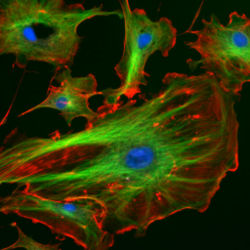
\includegraphics[width=0.5\linewidth]{images/250px-BMC_Cytoskeleton.jpg}}
    \caption{The eukaryotic cytoskeleton. Actin filaments are shown in red, microtubules in green, and the nuclei are in blue.}
    \label{fig:250px-BMC_Cytoskeleton}
\end{figure}

In this part of the experiment, you will observe the motion of particles inside a living cell. Cells transport food, waste, information, etc. in membrane-bound vesicles, which are visible under a light microscope. An old-fashioned view of a cell was that it is a ``bag of water'' containing various enzymes in which matter is transported passively by diffusion. Though diffusion is an important mechanism, it is too slow and random for long distance transport and directing materials where they are most needed, especially in larger cells. It is now understood that cells have highly developed and intricate mechanisms for directed transport of materials.

Most motions within and of cells involve two components, a cytoskeletal fiber that serves as a track, and a \href{http://physics111.lib.berkeley.edu/Physics111/Reprints/OTZ/biowikipedia.pdf}{\textbf{motor protein}} that does the work. The motor molecule uses energy from the hydrolysis of one ATP molecule to bind to the fiber, bend to pull itself along the fiber, and release, all of which constitutes one ``step''. For an animation of this stepping process, see this \href{https://valelab.ucsf.edu/molecular-animations/}{\textbf{movie animation}} from the Vale lab web site at UC San Francisco. One can divide cellular motility mechanisms into two classes based on the cytoskeletal fibers involved. (1) Microtubule-based mechanisms involve dynein or kinesin motors pulling on microtubules made of the protein tubulin. (2) Actin-based mechanisms involve myosin motors pulling on actin fibers, also called microfibers.

\begin{figure}[h]
\begin{minipage}[t]{.475\textwidth}
    \centering
    \href{http://experimentationlab.berkeley.edu/sites/default/files/images/Myosin.gif}{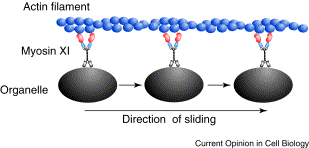
\includegraphics[width=\linewidth,keepaspectratio]{images/Myosin.png}}
    \caption{Cartoon of myosin motors pulling organelles along an actin filament.}
\end{minipage}\hfill
\begin{minipage}[t]{.475\textwidth}
    \centering
    \href{http://experimentationlab.berkeley.edu/sites/default/files/images/196px-Kinesin.jpg}{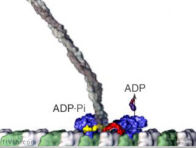
\includegraphics[width=\linewidth,keepaspectratio]{images/196px-Kinesin.jpg}}
    \caption{Binding of kinesin motor to microtubule.}
\end{minipage}
\end{figure}

Virtually all cell types exhibit directed intracellular transport, but some cell types are particularly suitable for transport studies. Fish-scale pigment cells work well, since a large fraction of the cargoes that are transported are pigmented and thus easy to observe – the disadvantage is that you would need to bring a living fish into lab as a source of these cells. For convenience, we will use epidermal cells from onion bulbs that you can easily acquire in a grocery store. With some care, a single layer of cells can be peeled off an inner section of the onion bulb and mounted flat on a slide.

\begin{figure}[h]
\begin{minipage}[t]{.475\textwidth}
    \centering
    \href{http://experimentationlab.berkeley.edu/sites/default/files/images/250px-Image005.png}{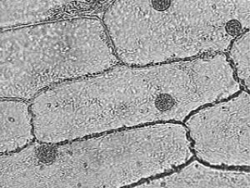
\includegraphics[width=\linewidth,keepaspectratio]{images/250px-Image005.png}}
    \caption{Onion cells in bright-field illumination. Round object in each cell is the nucleus.}
\end{minipage}\hfill
\begin{minipage}[t]{.475\textwidth}
    \centering
    \href{http://experimentationlab.berkeley.edu/sites/default/files/images/Image003.png}{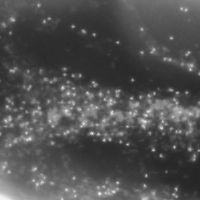
\includegraphics[width=\linewidth,keepaspectratio]{images/Image003.png}}
    \caption{Vesicles in the cytoplasm of a plant cell, as seen in dark-field.}
\end{minipage}
\end{figure}

In this experiment, we will be viewing the movement of vesicles within the cytoplasm of onion epidermal cells, shown above as they appear in bright-field and dark-field microscopy. The layers you see in an onion bulb develop into leaves when it sprouts. Both sides of the leaf are covered with an epidermis consisting of brick-shaped cells, each with a cell wall and cell membrane on the outside. Most of the interior of the cell is filled with a clear \href{http://en.wikipedia.org/wiki/Vacuole}{\textbf{vacuole}} that functions in storage and in maintenance of hydrostatic pressure essential to the stiffness of the plant (the difference between crisp lettuce and wilted lettuce). The \href{http://en.wikipedia.org/wiki/Cytoplasm}{\textbf{cytoplasm}}, containing all of the other cell contents, occurs in a thin layer between the cell membrane and the vacuole, and in thin extensions through the vacuole called transvacuolar strands. It is within the cytoplasm that you will be observing directed transport of vesicles by an actin-based mechanism. These vesicles are spherical or rod-shaped organelles such as mitochondria, spherosomes, and \href{http://en.wikipedia.org/wiki/Peroxisome}{\textbf{peroxisomes}} ranging in size from 0.5 to 3 microns. The diagram of an onion cell below shows the location of the cell wall, cytoplasm and vesicles in a typical cell; you will not be able to see much of the endoplasmic reticulum or the vacuole depicted because of their transparency. Under the microscope, you will notice the vesicles are located just along the edges of the cell, or near the top and bottom surface if you focus up and down. When you see a narrow band of moving vesicles in the center of the cell, it is located in a transvacuolar strand, which may be a handy place to study motion.

\begin{figure}[h]
    \centering
    \href{http://experimentationlab.berkeley.edu/sites/default/files/images/500px-BMC_OnionStucture.gif}{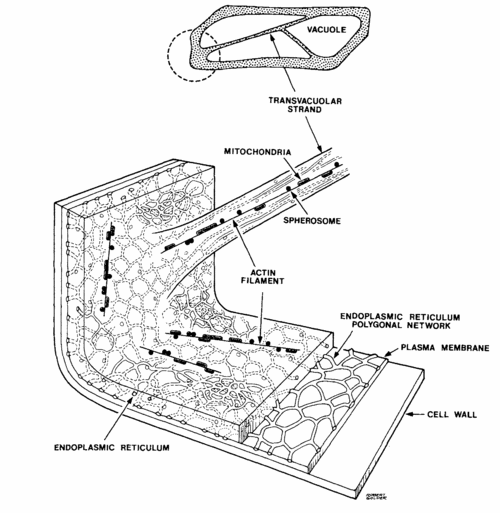
\includegraphics[width=0.5\linewidth]{images/500px-BMC_OnionStucture.png}}
    \caption{A 3D cross-section model of an onion epidermal cell, showing actin filaments and vesicles in the narrow bands of cytoplasm within the cell.}
    \label{fig:500px-BMC_OnionStucture}
\end{figure}

In plant cells, vesicles are transported along actin fibers by myosin motor molecules. An actin filament is composed of two intertwined actin chains, about 7 nm in diameter. An actin fiber is considered structurally polar, having a (+) end and a ($-$) end, and most myosin motors move only towards the (+) end of the actin fiber. In order to reverse the direction of a vesicle's motion, the vesicle must grab on to another actin fiber oriented in the opposite direction. There are at least eighteen described classes of myosin, of which three, myosin VIII, XI, and XII are found in plant cells. Some myosin motors are processive, meaning that they remain bound to an actin fiber as they move step-by-step along it (analagous to this \href{https://vimeo.com/157524451}{\textbf{movie animation of kinesin}}. Other myosins are non-processive, releasing from the actin fiber after each step. Myosin II found in muscle cells is non-processive, as illustrated in this \href{http://www.banyantree.org/jsale/actinmyosin/index.html}{\textbf{video animation}}. In the muscle functional unit, there are many myosin motors acting together, so there are always some attached to the actin fiber. The myosin XI responsible for transport of plant cell vesicles is the fastest myosin known and is processive. It is not certain how many myosin molecules are attached to the surface of a vesicle or how many of those are active at one time in pulling the vesicle along an actin fiber.

In some plant cells and algal cells, a large-scale streaming motion of the cytoplasm is observed, logically called \href{http://en.wikipedia.org/wiki/Cytoplasmic\_streaming}{\textbf{cytoplasmic streaming}}. This bulk flow is believed to be caused by myosin motors pulling the extensive endoplasmic reticulum along actin fibers lining the cell membrane. Many other vesicles are then dragged along with the endoplasmic reticulum. \href{http://www.ncbi.nlm.nih.gov/books/bv.fcgi?rid=mcb.figgrp.5242}{\textbf{Lodish and Berk, et al.}} provide a detailed explanation of this process and a video of cytoplasmic streaming in the pond weed Elodea can be viewed \href{http://www.microscopy-uk.org.uk/mag/imgnov00/cycloa3i.avi}{\textbf{here}}.

In your observations of vesicles in onion epidermal cells, you should distinguish between the random Brownian motion of vesicles that are unattached (or at least not actively moving along) actin filaments, the directed transport of vesicles by attached myosin motors, and possibly (though we are not sure this really happens in onions) bulk flow of vesicles in cytoplasmic streaming.

\subsection{Methods}

\subsubsection{Making an onion slide}

\begin{itemize}
    \item Before coming to lab obtain an onion from your favorite produce store. If you have forgotten one you can try the Seven Palms deli located conveniently at Euclid and Ridge, perhaps a five minute walk from LeConte.

    \item Use a knife, box-cutter, razorblade or whatever other cutting tool is provided to cut out a half-inch cube from the onion.

    \item Take one of the lower layers (activity depends somewhat on depth) and remove the lower membrane using the forceps, this is similar to pulling off a sticker. The easier it peels off, the less damage to the cells, so try several.

    \item The membrane is a single layer of cells which makes it particularly clean when viewing through a microscope. It should appear translucent and should be relatively strong.

    \item Make a slide using this membrane

    \begin{itemize}
        \item Place a drop of saline solution (contact lens solution works well) onto a clean slide (\emph{don't use water})

        \item Place the membrane onto the drop of saline on the slide

        \item Drop another drop onto the onion and cover with a cover slip

        \item Blot excess liquid using a paper towel

    \end{itemize}

    \item Mount onto microscope

    \item Keep in mind that the lifetime of an onion slide is about 30-60 minutes before it dries out.

    \item Put the remainder part of the onion into a plastic baggy and put it into the refrigerator.

    \item For the benefit of all future users of the refrigerator, please remove your onion when you have finished the lab. Do not leave it for the next group.

\end{itemize}

\subsubsection{Observing cells and trapping vesicles}

Scan the slide to find regions where cells aren't covered by air bubbles or badly damaged. Look for cells with an intact nucleus and some non-random motions of small vesicles. Occasionally a preparation will not show good motion and you should try another slide.

Examine patterns of motion within a cell. Some regions will show little activity, others will have large numbers of vesicles in motion. To study internal transport along actin filaments it will be helpful to find relatively isolated tracks along which small numbers of vesicles travel. Try trapping vesicles and see what happens to the movement of other vesicles along the same track. How does the vesicle behave when it is released? With a vesicle trapped, you can try moving it through the cytoplasm by moving the stage.

\subsection{Your Investigation}

Here are some ideas you could try:

\begin{enumerate}
    \item How do vesicles in active transport respond to manipulation by the trap? Does stopping and releasing a vesicle result in resumed motion, motion in the opposite direction, or ceasing of motion? What effect does trapping a vesicle have on other vesicles travelling the same route?

    \item Calibrate the trap stiffness using a vesicle. Many of the vesicles are similar in size to the beads you've used for calibration, but the vesicle's optical properties and the viscosity of the cytoplasm differ from the beads in water you used. By trapping a vesicle that is showing Brownian motion (not active transport), you could use the PSD method to estimate sensitivity and stiffness. (You will have to find a value from the literature for the viscosity of the cytoplasm to do your sensitivity calibration.) Or use the Equipartition method for stiffness and assume the same sensitivity you obtained with a bead. How does this compare with values obtained with beads in water?

    \item Measure the velocity of vesicles in active transport. If you set the laser power low enough that it doesn't appreciably slow down motion of vesicles in internal transport and position the trap so that a vesicle passes through the center (preferably in the X or Y direction), then you can use the QPD vs. time plot to estimate the speed of the vesicle. You can use the particle tracker software to make independent measurements of velocities (see the Brownian Motion in Cells lab for more details on this).

    \item Measure forces involved in active transport of vesicles. If the laser power is high enough to retard motion of the vesicle but not stop it, you might be able to use the QPD output vs. time to calculate the force that the trap is exerting on the vesicle. Or you might stop a vesicle and then reduce laser power until the vesicle can break free and look at the QPD reading at this power. This may be tricky to do. How do these measurements compare with the Stokes drag force calculated using vesicle size, velocity, and cytoplasm viscosity?

\end{enumerate}


\textbf{This is a Checkpoint: Complete at least two sets of questions. Call over a Professor or GSI and discuss the questions and the methods you will be using to tackle them. }

\section{Part IV: (Not Available) Measuring the Stall Force of Dynein Motor Molecules}

\emph{\textbf{Note that at this time this part of the lab cannot be done because we do not have a source for Dynein!}}

Before you can begin this experiment, ask Don Orlando to pick up several aliquots of the dynein motor protein. The dynein must then be kept on dry ice until ready for use.  Note: Please check whether any of the other materials are out of supply so that Don can pick up more when they get the dynein motors.

\subsection{Function of Dynein Within a Cell}

\begin{figure}[h]
    \centering
    \href{http://experimentationlab.berkeley.edu/sites/default/files/images/150px-Dynein_Motor.gif}{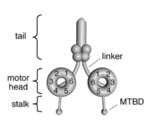
\includegraphics[width=0.5\linewidth]{images/150px-Dynein_Motor.png}}
    \caption{A dynein motor, consisting of a tail and two heads, each with an attached stalk.}
    \label{fig:150px-Dynein_Motor}
\end{figure}

Dynein is a eukaryotic motor protein that is involved in the transport of organelles, mRNA, and in the formation of mitotic spindles. The motor molecule consists of a tail, which binds to the cellular cargo, and two heads. A stalk extends from each head which can then bind to, and walk along, microtubules. Each head moves symmetrically in a hand-over-hand fashion, taking 8-32 nm steps. Dynein is also minus-end directed, which means that it preferentially walks towards the minus-end of the microtubule. However, it displays rather weak directionality as compared to other motor proteins, so it can often be observed to walk towards the plus-end as well. Dynein also remains attached to the microtubule when subject to a stall force for much longer than other motor proteins, even for up to several minutes before falling off. Both of these characteristics are thought to enable a tug-of-war type behavior in which multiple dynein molecules oriented towards opposite ends of a microtubule can collectively dictate the direction of transport. Also, the long stall time may bring stability to a transport process if the force force exerted on the dynein proteins occasionally exceeds their stall force.

\subsection{Methods}

\begin{figure}[h]
    \centering
    \href{http://experimentationlab.berkeley.edu/sites/default/files/images/200px-Dynein_On_Axoneme.gif}{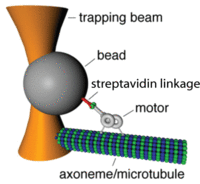
\includegraphics[width=0.3\linewidth]{images/200px-Dynein_On_Axoneme.png}}
    \caption{A dynein motor walking along an axoneme. The dynein head is bound to a microsphere, which is being pulled out of the optical trap.}
    \label{fig:200px-Dynein_On_Axoneme}
\end{figure}

Although dynein cannot be directly manipulated with an optical trap, we can promote binding between a silica bead and a dynein molecule such that the bead position can be used as a proxy for the actual dynein position. We do this by using beads coated with Streptavidin, which has a high affinity for the tails of dynein molecules. Once a bead/dynein structure has been trapped, it can be placed above an axoneme (microtubule bundle) to allow the dynein heads to bind. The dynein molecule can then begin walking towards the minus-end of the axoneme, pulling the bead out of the center of the trap. Eventually the force exerted on the trap will match the stall force of the dynein, and the dynein will stall. This can be seen as a plateau in the QPD voltage readout plot, and after a time you may see a sharp drop off, indicative of a stall and snap-back. You can then use this data to determine the stall force of individual dynein molecules.

\subsubsection{Slide Preparation}

Once you have received several aliquots of dynein motors from Don, \href{http://experimentationlab.berkeley.edu/sites/default/files/images/Dynein\_OTZ\_Slide\_Prep-Yildiz\_Lab.pdf}{\textbf{See the Dynein Prep Sheet}} you can put together the rest of the ingredients. Find the blue ice bucket in the cabinet and fill it up at the ice machine in room 151. All the materials you need can be stored in this bucket for the day. In the freezer in room 287, there will be several white cardboard boxes in which you should find the following:

\begin{itemize}
    \item ATP - Phosphorylated by dynein, provides the energy for stepping. Cannot be refrozen, throw out at end of day.

    \item PCD \& PCA - Scavenge oxygen that could be excited by the trapping laser into reactive oxidative species that weaken the bead/dynein bond and destabilize fluorescent dyes. Can be refrozen, PCA turns dark yellow when it is no longer useable.

    \item DTT - Reducing agent that prevents unwanted disulfide bonds forming between dynein motors and the axonemes. Can be refrozen $\sim$4 times, defrost vials of smaller quantities if possible.

    \item Axonemes - Ring of microtubules that provides binding sites for the dynein heads to step along. Can be refrozen.

\end{itemize}

\emph{Note: There will only be a few microliters of stock in some of the vials. This will be enough for your experiment.}

In the OTZ fridge, you can find the following materials:

\begin{itemize}
    \item Casein

    \item DLB Buffer

    \item Streptavidin-Coated Microspheres

\end{itemize}

The dynein aliquots are only useable for four hours after being defrosted, and cannot be refrozen. Keep one tube of dynein that you plan to use for the day in the ice bucket, but leave any remaining tubes in the dry ice.

Now that all the necessary ingredients are in the ice bucket, you may begin preparing the test sample. First, review the pipette and slide preparation instructions above. You will be dealing with very small volumes, so you will have to be thorough about mixing the solutions (since they are viscous) and not introducing many air bubbles into the solutions. Also, pipette the smaller components of a solution first.

\begin{enumerate}
    \item Prepare 150 $\mu$L of DLBC - In a 5 mL tube, mix 10 $\mu$L of Casein with 140 $\mu$L of DLB Buffer. Label with a sharpie, and place in the ice bucket. Repeat this last step for every solution you will make.

    \item Prepare motor dilution - Mix 1 $\mu$L of the dynein stock with 4 or more $\mu$L of DLBC. It is recommended that you start with a high concentration of dynein, and then decrease the concentration with each successive test sample you prepare. Ideally you will find a concentration at which enough beads have a single motor attached, but not multiple.

    \item As described in the slide assembly section, make a 1:10,000 dilution of Streptavidin-coated beads.

    \item Mix 2 $\mu$L of the bead solution with 2 $\mu$L of the motor solution, and place in the ice bucket for 10 minutes.

    \item Meanwhile, make the channel slide as described in the slide assembly above. The channel should be 2-3 mm wide.

    \item Prepare the axoneme solution - Mix 1 $\mu$L of axoneme stock with 6 $\mu$L of DLB (no casein). Mix as thoroughly as possible, since the glycerol content of the DLB does not mix easily.

    \item Prepare the stepping buffer-
    \begin{itemize}
        \item 1 $\mu$L PCA
    
        \item 1 $\mu$L PCD
    
        \item 1 $\mu$L ATP
    
        \item 1 $\mu$L DTT
    
        \item 2.5 $\mu$L DLB
    
        \item 3.5 $\mu$L Casein
    \end{itemize}

    \item After ten minutes has passed (don't worry if you took a little longer than that), add 14 $\mu$L of DLB and 2 $\mu$L of stepping buffer to the motor+beads solution.

    \item Place the slide against an object (like the coverslip box) such that the channel is tilted up, and slowly pipette all the axoneme solution into the channel.

    \item Do the same with the 20 $\mu$L of motor+bead+DLB+stepping buffer solution. You may have to simultaneously place the edge of a kimwipe against the lower edge of the channel to suck out the previous axoneme solution to fit the new solution.

    \item Seal the ends with nail polish.
\end{enumerate}

You can continue using the original motor solution (without beads), DLBC, and bead solution for any other tests you do during the four hours after the dynein was defrosted. However, the stepping buffer is only good for an hour, so it and the axoneme solution must be remade before every test.

\subsubsection{Trap Operation}

\begin{itemize}
    \item Once the slide is complete and placed upon the stage, you can begin the experiment. First, you may want to get a feel for what the axonemes look like. They are attached to the coverslip, and roughly in focus when the trap focus is about ten microns above the coverslip (you can trap a bead quickly to find the coverslip height). To find some axonemes, you will need to put in the emission filter, turn off all the lasers/illumination EXCEPT the green laser, and turn the shutter speed on the CCD to the slowest setting. They should appear as long strands, mostly oriented in the x direction. Once you have found them, you can turn on the illuminator and adjust the illuminator voltage and CCD shutter speed until you can see the beads and the axonemes. Alternatively, if the frame rate is too slow for your liking, you can try finding the axonemes using the illuminator only (at a brighter setting), and ignore the fluorescence.

\end{itemize}

\begin{itemize}
    \item Next, trap a bead, and move it over a roughly horizontal or vertical axoneme. Lower the bead until it barely goes out of focus. The dynein motor is only 25nm long, so the only way to ensure contact between it and the axoneme with our set-up is to rest the bead on top of the axoneme. However, if it is pushed too hard against the axoneme, the bead will be pushed to one side of the trap and provide incorrect results. The OTKB settings should be as follows:

\end{itemize}

Sample Rate = 1000 Hz

History Length = 120 Seconds

Diameter = 1.01 Microns (Unless the bead container says otherwise)

Viscosity = 1.2 Pa*s*1e-3 (Glycerol in DLB buffer increases the viscosity over water's)

You may set the QPD y-axis range as you wish, and turn off either the QPD X or Y display with the check button if you only want to see the output of one. You can also change the QPD Display units if you have roughly accurate values in the \emph{Calibrations} panel (does not affect data that is saved).

\begin{itemize}
    \item Watch the QPD display for two minutes to see if there is any motor activity. The bead freely rotates within the trap, so it may take up to two minutes for the dynein motor to contact the axoneme. If it does, save the two minute window with \emph{Save Voltage Data and Graph,} and save 3-4 more intervals of data if you see examples of dynein stalls. You can later go back and splice the data together in Matlab. Especially in the first few tests, however, it is likely that you have more than one motor attached to a given bead, and you won't see clean stall/detachment events. The bead may move out of the trap until one motor falls off the axoneme, but will not snap back all the way if another is still attached. To the right is an example of bead movement due to multiple motors. On the other hand, if the dynein concentration in the original motor solution was much too high, there may be so many motors on a bead that the motors stick to the axoneme, but cannot move. In this case, you will not see any activity, but upon turning the trapping laser off you will notice the bead is firmly attached to the axoneme.

    \begin{figure}[h]
        \centering
        \href{http://experimentationlab.berkeley.edu/sites/default/files/images/Dynein-Stall-Graph_No-Y-Axis.gif}{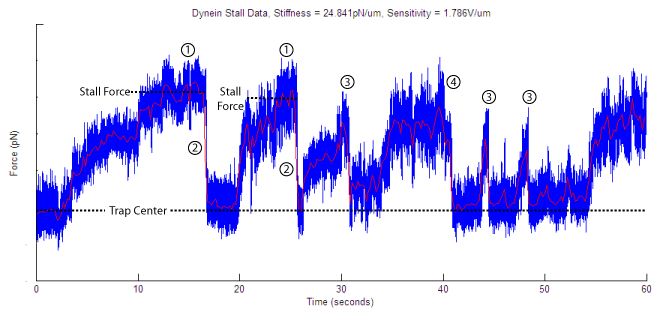
\includegraphics[width=0.9\linewidth]{images/Dynein-Stall-Graph_No-Y-Axis.png}}
        \caption{Force exerted by the optical trap upon a bead and motor, plotted against time. There are two stall events in this 60 second window. 1) Once the dynein motor reaches its stall force, the QPD output will plateau for a time. This is necessary prerequisite of any stall event. 2) After the plateau, the motor will detach and the bead will snap back to the center of the trap. A clean detachment is also a prerequisite of a stall event. 3) These three detachments display no prior plateau. They are likely due to random fluctuations in the system that provide the disassociation energy for the dynein motor, and do not count as stalls. 4) In this detachment event, the motor does not plateau but rather begins walking backwards to the center of the trap. It also is not considered a proper stall event.}
        \label{fig:Dynein-Stall-Graph_No-Y-Axis}
    \end{figure}

    \item After saving sufficient voltage data for a bead, drag it away from the axoneme and perform the PSD calibration upon it as described earlier. MAKE SURE TO CHANGE THE SAMPLE RATE AND HISTORY LENGTH ACCORDINGLY. To save time, just click \emph{Fit PSD and Save Data/Graph.} This will compute all the necessary calibration values you will need, available in the ``PSD Settings'' text file. Since the program automatically adds an different extension to your file name depending on which save button you click, you can enter the same name as you used for saving the voltage data (``Slide2\_Bead5'' for example) so you can easily match calibration data with voltage data later.

    \begin{figure}[h]
        \centering
        \href{http://experimentationlab.berkeley.edu/sites/default/files/images/150px-Gennerich_Stall_Data.jpg}{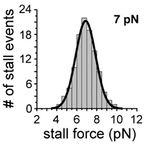
\includegraphics[width=0.3\linewidth]{images/150px-Gennerich_Stall_Data.jpg}}
        \caption{Histogram of dynein stall forces from Gennerich et al. 2007.}
        \label{fig:150px-Gennerich_Stall_Data}
    \end{figure}

    \item Keep track of how many beads show any activity. You should aim to measure at least 5-10 beads in each hour long trial.
    
    \emph{What proportion of beads should show no activity such that there is a 95\% probability an active bead only has one motor? Aim for this proportion.}

    \item In every subsequent slide you prepare, you should lower the concentration of the dynein solution until you are confident you are getting single-motor stall data. If you don't see any movement you may want to redo all the solution and try another slide.

    \item After you have found a workable concentration of dynein motors and have enough stall data saved, you can start compiling all the stall events you have from that trial. Ten stall events would be ideal, so it is possible you can get all your final data from a single trial, but you may need to repeat the experiment at the same dynein concentration if you don't think you have enough stall events saved.

    \item You will at the very least have to come up with an average value for the dynein stall force (there is currently no accurate published value), but beyond that it is up to you how you wish to present your data. You can simply compile all stall measurements into a histogram, or average the stalls from each individual bead first and plot those averages. You may also explore the spread of spontaneous drop-offs, when the motor detaches from the axoneme but shows no stall first. If the probability of a spontaneous drop-off is uncorrelated with force you may expect an exponential decay distribution, but it could easily be a much more complex distribution. Have fun with it! At this point, it is likely you have a better estimate of dynein stall force than the current published value, so you have just performed some very cutting-edge research!

    \item Last day of the experiment please fill out the \href{\ExperimentEvaluation}{\textbf{Experiment Evaluation}}
\end{itemize}

\begin{thebibliography}{}
\label{sec:References}
    \bibitem{Ashkin1970} \href{http://physics111.lib.berkeley.edu/Physics111/Reprints/OTZ/Acceleration_and_Trapping156_1.pdf}{\textbf{Arthur Ashkin, ``Acceleration and trapping of particles by radiation pressure'', Phys. Rev. Let. \textbf{24}(4), 156 (1970)}}. This is the original paper debuting the practice of optical trapping using two opposing lasers.

    \bibitem{Ashkin1997} \href{http://physics111.lib.berkeley.edu/Physics111/Reprints/OTZ/Ashkin-Optical-Trapping.pdf}{\textbf{\textbf{Arthur Ashkin, Optical trapping and manipulation of neutral particles using lasers}, Proc. Natl. Acad. Sci. \textbf{94},4853 (1997).}}Ashkin describes his discovery of optical trapping and how it was developed into tools of atom trapping and optical tweezers widely used in physics and biology.

    \bibitem{Leonardo} Trap forces applet by Roberto Di Leonardo, CNR-IPCF Dipartimento di Fiscica, Universita di Roma Sapienza

    \bibitem{Neuman} \href{http://physics111.lib.berkeley.edu/Physics111/Reprints/OTZ/Neuman-optical_Trapping.pdf}{\textbf{K. C. Neuman and S. M. Block, ``Optical Trapping,'' Rev. Sci. Instrum. \textbf{75}, 2787 (2004)}}

    \bibitem{Bechhoefer} \href{http://physics111.lib.berkeley.edu/Physics111/Reprints/OTZ/Bechhoefer_Wilson_Optical-Tweezers.pdf}{\textbf{J. Bechhoefer, S. Wilson, ``Faster, cheaper, safer optical tweezers for the undergraduate laboratory'', Am. J. Phys., \textbf{70}, 393 (2002)}}. Concise summary of optical trapping theory. Explores trapped particle theory using Equipartition method in considerable detail.

    \bibitem{Shaevitz} \href{http://physics111.lib.berkeley.edu/Physics111/Reprints/OTZ/OT_Practicle_Guide.pdf}{\textbf{J. W. Shaevitz, A practical guide to optical trapping}}, A concise guide to physics of trapping, principles of trap building, and theory and practical issues of trap calibration. Written while Shaevitz was a Miller Postdoc Fellow at Berkeley - he is now a professor at Princeton.

    \bibitem{Gittes} \href{http://www.opticsinfobase.org/ol/abstract.cfm?uri=ol-23-1-7}{\textbf{F. Gittes and C. F. Schmidt, Interference model for back-focal-plane displacement detection in optical tweezers. Optics Letters, \textbf{23}, 7 (1998)}}. Derivation of theory explaining the response of the quadrant photodiode to displacements of the trapped object.

    \bibitem{Reif} F. Reif, \emph{Fundamentals of Statistical and Thermal Physics}, McGraw Hill, New York, 1965. A useful reference, available in the physics library, for understanding the autocorrelation function and Power Spectrum Density: Chap. 15, especially Secs. 6 and 10.
\end{thebibliography}

Other References

\begin{enumerate}
    \item R. Pastel \emph{et al}., ``\href{http://physics111.lib.berkeley.edu/Physics111/Reprints/OTZ/Build-Optical-Trap-3.pdf}{\textbf{Laser trapping of microscopic particles for undergraduate experiments}}'', Am. J. Phys. \textbf{68,} 993 (2000)

    \item Other reprints and materials can be found on the \href{http://physics111.lib.berkeley.edu/Physics111/Reprints/OTZ/OTZ\_index.html}{\textbf{Physics 111 Library Site}}

    \item \href{http://experimentationlab.berkeley.edu/sites/default/files/images/Cable\_Diagram\_Laser\_TEC.pdf}{\textbf{Cable wiring diagram for SRS Laser \& TEC controller}}
\end{enumerate}

\end{document}
